\documentclass{amsart}

\usepackage{setspace}
\onehalfspacing

% \usepackage{fontspec}
% \setmainfont{Libertinus Serif}
% \setsansfont{Libertinus Sans}
% \setmonofont{Liberation Mono}

\usepackage[style=alphabetic, backref, giveninits, maxbibnames=10]{biblatex}
\addbibresource{o-minimal.bib}

\usepackage{graphicx}
\usepackage{xcolor}
\usepackage{amsmath, amsfonts, amssymb, mathtools, amsthm}
\usepackage{enumitem}
\usepackage{hyperref}
\usepackage{xurl}

\usepackage{tikz}
\usetikzlibrary{shapes.geometric,arrows,cd}

\tikzstyle{notions} = [rectangle, rounded corners,
minimum width=3cm,
minimum height=1cm,
text centered,
draw=black,
fill=white!30]
\tikzstyle{arrow} = [thick,->,>=stealth]

\usepackage{tcolorbox}

\newtheorem{theorem}{Theorem}[subsection]
\newtheorem{lemma}[theorem]{Lemma}
\newtheorem{proposition}[theorem]{Proposition}
\newtheorem{corollary}[theorem]{Corollary}
\newtheorem{construction}[theorem]{Construction}

\theoremstyle{definition}
\newtheorem{definition}[theorem]{Definition}
\newtheorem{remark}[theorem]{Remark}
\newtheorem{example}[theorem]{Example}
\numberwithin{equation}{section}

\newcommand{\definable}{\mathrm{def}}
\newcommand{\analytic}{\mathrm{an}}


\title{Notes on o-minimality}
\author{Tang Zhichao}
\author{Chen Zaiyuan}
\date{\today}

\begin{document}

\maketitle

\tableofcontents

\section{Basic model theory}
Materials follow from \cite{zbMATH01821671,zbMATH01160037},
mainly \cite{zbMATH01821671}.
\subsection{Languages and Structures}
The goal of this section is to describe what is o-minimality
from a model theoretic aspect,
therefore some logical preliminaries are required.
Some standard theory related to the real numbers
will be proved to be o-minimal,
not only about polynomials, but can include the exponential function and analytic functions.

\subsubsection{Basic definitions}
In mathematical logic,
we use first-order languages to describe mathematical structures.
Intuitively, a structure is a set that we wish to study equipped with a collection of distinguished functions, relations, and elements.
We then choose a language where we can talk about the distinguished functions, relations, and elements and nothing more.

\begin{definition}
	A \emph{language $\mathcal{L}$} is given by specifying the following data:
	\begin{enumerate}[label = {(\roman*)}]
		\item a set of function symbols $\mathcal{F}$ and positive integers $n_f$ for each $f \in \mathcal{F}$;
		\item a set of relation symbols $\mathcal{R}$ and positive integers $n_R$ for each $R \in \mathcal{R}$;
		\item a set of constant symbols $\mathcal{C}$.
	\end{enumerate}
\end{definition}

\begin{definition}
	An \emph{$\mathcal{L}$-structure $\mathcal{M}$} is given by the following data:
	\begin{enumerate}[label = {(\roman*)}]
		\item a nonempty set $M$ called the universe, domain, or underlying set of $\mathcal{M}$;
		\item a function $f^{\mathcal{M}} : M^{n_f} \to M$ for each $f \in \mathcal{F}$;
		\item a set $R^{\mathcal{M}} \subseteq M^{n_R}$ for each $R \in \mathcal{R}$;
		\item an element $c^{\mathcal{M}} \in M$ for each $c \in \mathcal{C}$.
	\end{enumerate}
\end{definition}

\begin{definition}
	Suppose that $\mathcal{M}$ and $\mathcal{N}$ are $\mathcal{L}$-structures with universes $M$ and $N$, respectively.
	An \emph{$\mathcal{L}$-embedding} is a one-to-one (injective) map $\eta: M \to N$
	that preserves the interpretation of all of the symbols of $\mathcal{L}$.
	\begin{enumerate}[label = {(\roman*)}]
		\item $\eta(f^{\mathcal{M}}(a_1,\dots,a_{n_f})) = f^{\mathcal{N}}(\eta(a_1),\dots,\eta(a_{n_f}))$
		      for all $f\in \mathcal{F}$ and $a_1,\dots,a_{n_f} \in M$;
		\item $(a_1,\dots,a_{n_R}) \in R^{\mathcal{M}}$ if and only if
		      $(\eta(a_1),\dots,\eta(a_{n_R})) \in R^{\mathcal{N}}$ for all $R \in \mathcal{R}$ and $a_1,\dots,a_{n_R} \in M$;
		\item $\eta(c^{\mathcal{M}}) = c^{\mathcal{N}}$ for all $c \in \mathcal{C}$.
	\end{enumerate}
	A bijective $\mathcal{L}$-embedding is called an \emph{$\mathcal{L}$-isomorphism}.
	If $M \subseteq N$ and the inclusion map is an $\mathcal{L}$-embedding,
	$\mathcal{M}$ is a \emph{substructure} of $\mathcal{N}$ or that
	$\mathcal{N}$ is an \emph{extension} of $\mathcal{M}$.
\end{definition}

The \emph{cardinality} of $\mathcal{M}$ is $|M|$,
the cardinality of the universe of $\mathcal{M}$.
If $\eta: \mathcal{M} \to \mathcal{N}$ is an embedding then
the cardinality of $\mathcal{N}$ is at least the cardinality of $\mathcal{M}$.

\begin{definition}
	The set of \emph{$\mathcal{L}$-terms} is the smallest set $\mathcal{T}$ such that
	\begin{enumerate}[label = {(\roman*)}]
		\item $c\in \mathcal{T}$ for each constant symbol $c \in \mathcal{C}$,
		\item each variable symbol $v_i \in \mathcal{T}$ for $i = 1,2,\dots$, and
		\item if $t_1,\dots,t_{n_f} \in \mathcal{T}$ and $f \in \mathcal{F}$, then $f(t_1,\dots,t_{n_f}) \in \mathcal{T}$.
	\end{enumerate}
\end{definition}

\begin{definition}
	$\phi$ is an \emph{atomic $\mathcal{L}$-formula} if $\phi$ is either
	\begin{enumerate}[label= {\roman*)}]
		\item $t_1 = t_2$, where $t_1$ and $t_2$ are terms, or
		\item $R(t_1,\dots,t_{n_R})$, where $R \in \mathcal{R}$ and $t_1,\dots,t_{n_R}$ are terms.
	\end{enumerate}
	The set of \emph{$\mathcal{L}$-formulas} is the smallest set $\mathcal{W}$ containing the atomic formulas such that
	\begin{enumerate}[label= {\roman*)}]
		\item if $\phi$ is in $\mathcal{W}$, then $\neg\phi$ is in $\mathcal{W}$,
		\item if $\phi$ and $\psi$ are in $\mathcal{W}$, then $(\phi \land \psi)$ and $(\phi \lor \psi)$ are in $\mathcal{W}$, and
		\item if $\phi$ is in $\mathcal{W}$, then $\exists v_i\, \phi$ and $\forall v_i\, \phi$ are in $\mathcal{W}$.
	\end{enumerate}
\end{definition}

A variable $v$ \emph{occurs freely} in a formula $\phi$
if it is not inside a $\exists v$ or $\forall v$ quantifier;
otherwise, it is \emph{bound}.
A formula is a \emph{sentence} if it has no free variables.

\begin{definition}
	Let $\phi$ be a formula with free variables from
	$\overline{v} = (v_{i_1},\dots,v_{i_m})$, and let
	$\overline{a} = (a_{i_1},\dots,a_{i_m})\in M^m$.
	Inductively define \emph{$\mathcal{M} \models \phi(\overline{a})$} as follows.
	\begin{enumerate}[label = {\roman*)}]
		\item If $\phi$ is $t_1 = t_2$, then $\mathcal{M} \models \phi(\overline{a})$
		      if $t_1^{\mathcal{M}}(\overline{a}) = t_2^{\mathcal{M}}(\overline{a})$.
		\item If $\phi$ is $R(t_1,\dots,t_{n_R})$, then $\mathcal{M} \models \phi(\overline{a})$
		      if $(t^{\mathcal{M}}_1(\overline{a}),\dots,t^{\mathcal{M}}_{n_R}(\overline{a})) \in R^{\mathcal{M}}$.
		\item If $\phi$ is $\neg \psi$, then $\mathcal{M} \models \phi(\overline{a})$ if $\mathcal{M} \not\models \psi(\overline{a})$.
		\item If $\phi$ is $(\psi \land \theta)$, then $\mathcal{M} \models \phi(\overline{a})$
		      if $\mathcal{M} \models \psi(\overline{a})$ and $\mathcal{M} \models \theta(\overline{a})$.
		\item If $\phi$ is $(\psi \lor \theta)$, then $\mathcal{M} \models \phi(\overline{a})$
		      if $\mathcal{M} \models \psi(\overline{a})$ or $\mathcal{M} \models \theta(\overline{a})$.
		\item If $\phi$ is $\exists v_j \psi(\overline{v},v_j)$, then $\mathcal{M} \models \phi(\overline{a})$
		      if there is $b \in M$ such that $\mathcal{M} \models \psi(\overline{a},b)$.
		\item If $\phi$ is $\forall v_j \psi(\overline{v},v_j)$,
		      then $\mathcal{M} \models \phi(\overline{a})$ if $\mathcal{M} \models \psi(\overline{a},b)$ for all $b \in M$.
	\end{enumerate}
	If $\mathcal{M} \models \phi(\overline{a})$ we say that
	$\mathcal{M}$ \emph{satisfies} $\phi(\overline{a})$ or $\phi(\overline{a})$ is \emph{true} in $\mathcal{M}$.
\end{definition}

\begin{proposition}
	Suppose that $\mathcal{M}$ is a substructure of $\mathcal{N}$,
	$\overline{a} \in M$, and $\phi(\overline{v})$ is a quantifier-free formula.
	Then, $\mathcal{M} \models \phi(\overline{a})$ if and only if $\mathcal{N} \models \phi(\overline{a})$.
\end{proposition}

\begin{definition}
	Two $\mathcal{L}$-structures $\mathcal{M}$ and $\mathcal{N}$ are \emph{elementarily equivalent}
	and denote $\mathcal{M} \equiv \mathcal{N}$ if
	\[
		\mathcal{M} \models \phi \text{ if and only if }\mathcal{N} \models \phi
	\]
	for all $\mathcal{L}$-sentences $\phi$.
\end{definition}

\subsubsection{Theories and logical consequence}
Let $\mathrm{Th}(\mathcal{M})$, the \emph{full theory} of $\mathcal{M}$,
be the set of $\mathcal{M}$-sentences $\phi$ such that $\mathcal{M} \models \phi$.

$\mathcal{M} \equiv \mathcal{N}$ if and only if $\mathrm{Th}(\mathcal{M}) = \mathrm{Th}(\mathcal{N})$.

\begin{theorem}
	Suppose that $j: \mathcal{M} \to \mathcal{N}$ is an isomorphism.
	Then, $\mathcal{M} \equiv \mathcal{N}$.
\end{theorem}

Let $\mathcal{L}$ be a language.
An \emph{$\mathcal{L}$-theory $T$} is a set of $\mathcal{L}$-sentences.

$\mathcal{M}$ is a \emph{model} of $T$ and denote $\mathcal{M} \models T$ if $\mathcal{M} \models \phi$ for all sentences $\phi \in T$.

A theory is \emph{satisfiable} if it has a model.

A class of $\mathcal{L}$-structures $\mathcal{K}$ is an \emph{elementary class}
if there is an $\mathcal{L}$-theory $T$ such that $\mathcal{K} = \{ \mathcal{M}:\mathcal{M} \models T \}$.
The sentences in $T$ are called \emph{axioms} for the elementary class.

\begin{definition}
	Let $T$ be an $\mathcal{L}$-theory and $\phi$ an $\mathcal{L}$-sentence.
	$\phi$ is a \emph{logical consequence} of $T$ and denote $T \models \phi$ if $\mathcal{M} \models \phi$
	whenever $\mathcal{M} \models T$.
\end{definition}

\subsubsection{Definability and Interpretability}
\begin{definition}
	Let $\mathcal{M} = (M,\dots)$ be an $\mathcal{L}$-structure.
	$X \subseteq M^n$ is \emph{definable} if and only if there is an $\mathcal{L}$-formula $\phi(v_1,\dots,v_n,w_1,\dots,w_m)$
	and $\overline{b} \in M^m$ such that $X = \{ \overline{a} \in M^n : \mathcal{M} \models \phi(\overline{a},\overline{b}) \}$.
	$\phi(\overline{v},\overline{b})$ \emph{defines} $X$.

	$X$ is \emph{$A$-definable }or \emph{definable over $A$} if there is a formula $\psi(\overline{v},w_1,\dots,w_l)$ and
	$\overline{b} \in A^l$ such that $\psi(\overline{v},\overline{b})$ defines $X$.
\end{definition}

\begin{lemma}
	Let $\mathcal{L}_r$ be the language of ordered rings and
	$(\mathbb{R}, +, -, \cdot, <, 0, 1)$ be the ordered field of real numbers.
	Suppose that $X \subset \mathbb{R}^n$ is $A$-definable.
	Then, the topological closure of $X$ is also $A$-definable.
\end{lemma}

\begin{proposition}[Concrete Characterization of Definable Sets]
	Let $\mathcal{M}$ be an $\mathcal{L}$-structure.
	Suppose that $D_n$ is a collection of subsets of $M^n$ for all $n \ge 1$ and
	$\mathcal{D} = (D_n : n \ge 1)$ is the smallest collection such that:
	\begin{enumerate}[label = {\roman*)}]
		\item $M^n \in D_n$;
		\item for all $n$-ary function symbols $f$ of $\mathcal{L}$, the graph of $f^{\mathcal{M}}$ is in $D_{n+1}$;
		\item for all $n$-ary relation symbols $R$ of $\mathcal{L}$, $R^{\mathcal{M}} \in D_n$;
		\item for all $i$, $j\le n$, $\{(x_1,\dots,x_n)\in M^n : x_i = x_j\} \in D_n$;
		\item if $X \in D_n$, then $M \times X \in D_{n+1}$;
		\item each $D_n$ is closed under complement, union, and intersection;
		\item if $X \in D_{n+1}$ and $\pi: M^{n+1} \to M^n$ is the projection map $(x_1,\dots,x_{n+1}) \mapsto (x_1,\dots,x_n)$,
		      then $\pi(X) \in D_n$;
		\item if $X \in D_{n+m}$ and $b \in M^m$, then $\{a\in M^n: (a,b) \in X \} \in D_n$.
	\end{enumerate}
	Then, $X \subseteq M^n$ is definable if and only if $X \in D_n$.
\end{proposition}

\begin{proposition}
	Let $\mathcal{M}$ be an $\mathcal{L}$-structure.
	If $X \subset M^n$ is $A$-definable,
	then every $\mathcal{L}$-automorphism of $\mathcal{M}$ that fixes $A$ pointwise fixes $X$ setwise.
\end{proposition}

\begin{definition}
	An $\mathcal{L}_0$-structure $\mathcal{N}$ is \emph{definably interpreted} in an $\mathcal{L}$-structure $\mathcal{M}$
	if and only if one can find a definable $X \subseteq M^n$ for some $n$ and can interpret the symbols of $\mathcal{L}_0$
	as definable subsets and functions on $X$ (definable using $\mathcal{L}$)
	so that the resulting $\mathcal{L}_0$-structure is isomorphic to $\mathcal{N}$.

	An $\mathcal{L}_0$-structure $\mathcal{N}$ is \emph{interpretable} in an $\mathcal{L}$-structure $\mathcal{M}$
	if there is a definable $X \subseteq M^n$, a definable equivalence relation $E$ on $X$,
	and for each symbol of $\mathcal{L}_0$, one can find definable $E$-invariant sets on $X$
	such that $X / E$ with the induced structure is isomorphic to $\mathcal{N}$.
\end{definition}

Let $S$ be a set.
The universe of a \emph{many-sorted structure} $\mathcal{N}$ with sorts $S$ is
a set $N$ that is partitioned into disjoint sets $\{N_i : i \in S\}$.
For each $n$-ary relation symbol $R$,
there are $s_1,\dots,s_n \in S$ such that $R^{\mathcal{N}} \subset N^{s_1} \times \dots \times N^{s_n}$.
For each $n$-ary function symbol $f$,
there are $s_0,\dots,s_n \in S$ such that $f^{\mathcal{N}} : N^{s_1} \times \dots \times N^{s_n} \to N^{s_0}$.

Let $\mathcal{M}$ be an $\mathcal{L}$-structure.
The set of sorts $S = \{S_E : E$ an $\emptyset$-definable equivalence relation on $M^n$ for some $n$ $\}$.
In the many-sorted structure $\mathcal{M}^{\mathrm{eq}}$,
one interpret the sort $S_E$ as $M^n / E$ for $E$ an $\emptyset$-definable equivalence relation on $M^n$.
Because $=$ is a definable equivalence relation on $M$,
$M$ can be identified with the sort $S_{=}$.
All relations and functions of $\mathcal{L}$ are relations and functions on $M^k$.
For each $\emptyset$-definable equivalence relation $E$ on $M^n$,
we have in $\mathcal{M}^{\mathrm{eq}}$ an $n$-ary function $f_E: M^n \to S_E$ given by $f_E(\overline{x}) = \overline{x} / E$.

\begin{lemma}
	\begin{enumerate}[label = {\roman*)}]
		\item If $X \subseteq M^n$ is definable in $\mathcal{M}^{\mathrm{eq}}$, then $X$ is definable in $\mathcal{M}$.
		\item If $\mathcal{M} \equiv \mathcal{N}$, then $\mathcal{M}^{\mathrm{eq}} \equiv \mathcal{N}^{\mathrm{eq}}$.
		\item If $\sigma$ is an automorphism of $\mathcal{M}^{\mathrm{eq}}$, then $\sigma|M$ is an automorphism of $\mathcal{M}$.
		\item If $\sigma$ is an automorphism of $\mathcal{M}$,
		      there is $\widehat{\sigma}$ an automorphism of $\mathcal{M}^{\mathrm{eq}}$ such that $\sigma = \widehat{\sigma}|M$.
	\end{enumerate}
\end{lemma}

\subsection{Basic Techniques and Important Results}
\subsubsection{Completeness and Compactness}
Let $T$ be an $\mathcal{L}$-theory and $\phi$ an $\mathcal{L}$-sentence.
A proof of $\phi$ from $T$ is a finite sequence of $\mathcal{L}$-formulas
$\psi_1,\dots,\psi_m$ such that $\psi_m = \phi$ and $\psi_i \in T$ or
$\psi_i$ follows from $\psi_1,\dots,\psi_{i-1}$ by a simple logical rule for each $i$.

Denote $T \vdash \phi$ if there is a proof of $\phi$ from $T$.

Some properties of the proof system:
\begin{enumerate}[label = {$\bullet$}]
	\item Proofs are finite.
	\item (Soundness) If $T \vdash \phi$, then $T \models \phi$.
	\item If $T$ is a finite set of sentences, then there is an algorithm that,
	      when given a sequence of $\mathcal{L}$-formulas $\sigma$ and an $\mathcal{L}$-sentence $\phi$,
	      will decide whether $\sigma$ is a proof of $\phi$ from $T$.
\end{enumerate}

A language $\mathcal{L}$ is \emph{recursive} if there is an algorithm that
decides whether a sequence of symbols is an $\mathcal{L}$-formula.
An $\mathcal{L}$-theory $T$ is recursive if there is a algorithm that,
when given an $\mathcal{L}$-sentence $\phi$ as input, decides whether $\phi \in T$.

\begin{theorem}[G\"odel's Completeness Theorem]
	Let $T$ be an $\mathcal{L}$-theory and $\phi$ an $\mathcal{L}$-sentence, then $T \models \phi$ if and only if $T\vdash \phi$.
\end{theorem}

\begin{definition}
	An $\mathcal{L}$-theory $T$ is \emph{inconsistent}
	if $T \vdash (\phi \land\neg\phi)$ for some sentence $\phi$;
	otherwise $T$ is \emph{consistent}.
\end{definition}

\begin{theorem}[Compactness Theorem]
	$T$ is satisfiable if and only if every finite subset of $T$ is satisfiable.
\end{theorem}

\begin{definition}
	A theory $T$ is \emph{finitely satisfiable} if every finite subset of $T$ is satisfiable.
\end{definition}

% \begin{definition}
%     An $\mathcal{L}$-theory $T$ has the \emph{witness property} if
%     whenever $\phi(v)$ is an $\mathcal{L}$-formula with one free variable $v$,
%     then there is a constant symbol $c \in \mathcal{L}$ such that
%     $T \models (\exists v\, \phi(v) \to \phi(c))$.
% \end{definition}

\begin{definition}
	An $\mathcal{L}$-theory $T$ is \emph{maximal} if for all $\phi$ either $\phi \in T$ or $\neg \phi \in T$.
\end{definition}

% \begin{lemma}
%     Suppose that $T$ is a maximal and finitely satisfiable $\mathcal{L}$-theory with witness property.
%     Then, $T$ has a model.
%     In fact, if $\kappa$ is a cardinal and $\mathcal{L}$ has at most $\kappa$ constant symbols, then there exists $\mathcal{M} \models T$ with $|\mathcal{M}| \le \kappa$.
% \end{lemma}

% \begin{lemma}
%     Let $T$ be a finitely satisfiable $\mathcal{L}$-theory.
%     There is a language $\mathcal{L}^* \supseteq \mathcal{L}$ and $T^* \supseteq T$ a finitely satisfiable $\mathcal{L}^*$-theory such that any $\mathcal{L}^*$-theory extending $T^*$ has the witness property.
%     $\mathcal{L}^*$ can be chosen such that $|\mathcal{L}^*| = |\mathcal{L}| + \aleph_0$.
% \end{lemma}

\begin{lemma}
	Suppose that $T$ is a finitely satisfiable $\mathcal{L}$-theory and $\phi$ is an $\mathcal{L}$-sentence, then,
	either $T \cup \{\phi\}$ or $T \cup \{\neg\phi\}$ is satisfiable.
\end{lemma}

\begin{corollary}
	If $T$ is a finitely satisfiable $\mathcal{L}$-theory,
	then there is a maximal finitely satisfiable $\mathcal{L}$-theory $T' \supseteq T$.
\end{corollary}

% \begin{theorem}
%   If $T$ is a finitely satisfiable $\mathcal{L}$-theory and $\kappa$ is an infinite cardinal with $\kappa \ge |\mathcal{L}|$,
%   then there is a model of $T$ of cardinality at most $\kappa$.
% \end{theorem}

% \begin{lemma}
%   If $T \models \phi$, then $\Delta \models \phi$ for some finite $\Delta \subseteq T$.
% \end{lemma}

\begin{definition}
	An $\mathcal{L}$-theory $T$ is called \emph{complete} if for any $\mathcal{L}$-sentence $\phi$,
	either $T \models \phi$ or $T \models \neg\phi$.
\end{definition}

% \begin{proposition}
%   Let $T$ be an $\mathcal{L}$-theory with infinite models.
%   If $\kappa$ is an infinite cardinal and $\kappa \ge |\mathcal{L}|$,
%   then there is a model of $T$ of cardinality $\kappa$.
% \end{proposition}

\begin{definition}
	Let $\kappa$ be an infinite cardinal and let $T$ be a theory with models of size $\kappa$.
	$T$ is \emph{$\kappa$-categorical} if any two models of $T$ of cardinal $\kappa$ are isomorphic.
\end{definition}

\begin{tcolorbox}
	Some abbreviation for commonly used theories:
	\begin{enumerate}[label = {}]
		\item \textbf{DLO}: dense linear order;
		\item \textbf{ACF}: algebraic closed field;
		\item \textbf{RCF}: real closed field;
		\item \textbf{DCF}: differential closed field.
	\end{enumerate}
\end{tcolorbox}

Let $\mathbf{ACF_p}$ be the theory of algebraically closed fields of characteristic $p$,
where $p$ is either $0$ or a prime number.

\begin{proposition}
	$\mathbf{ACF}_p$ is $\kappa$-categorical for all uncountable cardinals $\kappa$.
\end{proposition}

\begin{theorem}[Vaught's Test]
	Let $T$ be a satisfiable theory with no finite models that is
	$\kappa$-categorical for some infinite cardinal $\kappa \ge |\mathcal{L}|$.
	Then $T$ is complete.
\end{theorem}

% \begin{definition}
%     An $\mathcal{L}$-theory $T$ is \emph{decidable} if there is an algorithm that
%     when given an $\mathcal{L}$-sentence $\phi$ as input decides whether $T \models \phi$.
% \end{definition}

% \begin{lemma}
%     Let $T$ be a recursive complete satisfiable theory in a recursive language $\mathcal{L}$.
%     Then $T$ is decidable.
% \end{lemma}

% \begin{corollary}
%     For $p = 0$ or $p$ prime, $\mathbf{ACF}_p$ is decidable.
% \end{corollary}

\begin{corollary}
	Let $\phi$ be a sentence in the language of rings.
	The following are equivalent.
	\begin{enumerate}[label = {\roman*)}]
		\item $\phi$ is true in the complex numbers.
		\item $\phi$ is true in every algebraically closed field of characteristic zero.
		\item $\phi$ is true in some algebraically closed field of characteristic zero.
		\item There are arbitrarily large primes $p$ such that $\phi$ is true in some algebraically closed field of characteristic $p$.
		\item There is an $m$ such that for all $p > m$, $\phi$ is true in all algebraically closed fields of characteristic $p$.
	\end{enumerate}
\end{corollary}

\subsubsection{Between structures}
\begin{definition}
	If $\mathcal{M}$ and $\mathcal{N}$ are $\mathcal{L}$-structures,
	then an $\mathcal{L}$-embedding $j: \mathcal{M} \to \mathcal{N}$ is called an \emph{elementary embedding} if
	\[
		\mathcal{M} \models \phi(a_1,\dots,a_n) \iff \mathcal{N} \models \phi(j(a_1),\dots,j(a_n))
	\]
	for all $\mathcal{L}$-formulas $\phi(v_1,\dots,v_n)$ and all $a_1,\dots,a_n \in M$.

	If $\mathcal{M}$ is a substructure of $\mathcal{N}$,
	it is called an \emph{elementary substructure} and
	denote $\mathcal{M} \prec \mathcal{N}$ if the inclusion map is elementary,
	equivalently, $\mathcal{N}$ is an \emph{elementary extension} of $\mathcal{M}$.
\end{definition}

\begin{definition}
	Suppose that $\mathcal{M}$ is an $\mathcal{L}$-structure.
	Let $\mathcal{L}_M$ be the language where we add to $\mathcal{L}$ constant symbols $m$ for each element of $M$.
	The \emph{atomic diagram} of $\mathcal{M}$ is
	$\{\phi(m_1,\dots,m_n):\phi$ is either an atomic $\mathcal{L}$-formula or the negation of an atomic $\mathcal{L}$-formula and $\mathcal{M} \models \phi(m_1,\dots,m_n)\}$.
	The \emph{elementary diagram} of $\mathcal{M}$ is
	\[
		\phi(m_1,\dots,m_n): \mathcal{M} \models \phi(m_1,\dots,m_n),\text{$\phi$ is an $\mathcal{L}$-formula}.
	\]
	Let $\mathrm{Diag}(\mathcal{M})$ and $\mathrm{Diag_el}(\mathcal{M})$ denote the atomic and elementary diagrams of $\mathcal{M}$, respectively.
\end{definition}

\begin{theorem}[Upward L\"owenheim--Skolem Theorem]
	Let $\mathcal{M}$ be an infinite $\mathcal{L}$-structure and
	$\kappa$ be an infinite cardinal $\kappa \ge |\mathcal{M}| + |\mathcal{L}|$.
	Then, there is $\mathcal{N}$ an $\mathcal{L}$-structure of cardinality $\kappa$ and $j: \mathcal{M} \to \mathcal{N}$ is elementary.
\end{theorem}

\begin{proposition}[Tarski--Vaught Test]
	Suppose that $\mathcal{M}$ is a substructure of $\mathcal{N}$.
	Then, $\mathcal{M}$ is an elementary substructure if and only if,
	for any formula $\phi(v,\overline{w})$ and $\overline{a} \in M$,
	if there is $b \in N$ such that $\mathcal{N} \models \phi(b,\overline{a})$,
	there is $c \in M$ such that $\mathcal{N} \models \phi(c,\overline{a})$.
\end{proposition}

% An $\mathcal{L}$-theory $T$ has \emph{built-in Skolem functions}
% if for all $\mathcal{L}$-formulas $\phi(v,w_1,\dots,w_n)$ there is a function symbol $f$
% such that $T \models \forall \overline{w} ((\exists v \phi(v,\overline{w})) \to \phi(f(\overline{w}),\overline{w}))$.
% In other words, there are enough function symbols in the language to witness all existential statements.

% \begin{lemma}
%   Let $T$ be an $\mathcal{L}$-theory.
%   There are $\mathcal{L}^* \supseteq \mathcal{L}$and $T^* \supseteq T$ an $\mathcal{L}^*$-theory
%   such that $T^*$ has built-in Skolem functions,
%   and if $\mathcal{M} \models T$,
%   then $\mathcal{M}$ can be expanded to $\mathcal{M}^* \models T^*$.
%   $\mathcal{L}^*$ can be chosen such that $|\mathcal{L}^*|= |\mathcal{L}|+\aleph_0$.

%   We call $T^*$ a skolemization of $T$.
% \end{lemma}

\begin{theorem}[L\"owenheim--Skolem Theorem]
	Suppose $\mathcal{M}$ is an $\mathcal{L}$-structure and
	$X \subseteq M$, there is an elementary submodel $\mathcal{N}$ of $\mathcal{M}$
	such that $X \subseteq N$ and $|\mathcal{N}| \le |X| + |\mathcal{L}| + \aleph_0$.
\end{theorem}

\begin{definition}
	A \emph{universal sentence} is one of the form
	$\forall \overline{v} \phi(\overline{v})$,
	where $\phi$ is quantifier-free.
	An $\mathcal{L}$-theory $T$ has a \emph{universal axiomatization} if there is a set of universal $\mathcal{L}$-sentences $\Gamma$
	such that $\mathcal{M} \models \Gamma$ if and only if $\mathcal{M} \models T$ for all $\mathcal{L}$-structures $\mathcal{M}$.
\end{definition}

\begin{theorem}
	An $\mathcal{L}$-theory $T$ has a universal axiomatization if and only if
	whenever $\mathcal{M} \models T$ and $\mathcal{N}$ is a substructure of $\mathcal{M}$,
	then $\mathcal{N} \models T$.
\end{theorem}

\begin{definition}
	Suppose that $(I,<)$ is a linear order.
	Suppose that $\mathcal{M}_i$ is an $\mathcal{L}$-structure for $i \in I$.
	$(\mathcal{M}_i: i \in I)$ is a \emph{chain} of $\mathcal{L}$-structures if $\mathcal{M}_i \subseteq \mathcal{M}_j$ for $i < j$.
	If $\mathcal{M}_i \prec \mathcal{M}_j$ for $i < j$,
	$(\mathcal{M}_i: i \in I)$ is an \emph{elementary chain}.
\end{definition}

\begin{proposition}
	Suppose that $(I,<)$ is a linear order and
	$(\mathcal{M}_i: i \in I)$ is an elementary chain.
	Then, $\mathcal{M} = \bigcup_{i\in I} M_i$ is an elementary extension of each $\mathcal{M}_i$.
\end{proposition}

\begin{definition}
	A theory $T$ has a \emph{$\forall\exists$-axiomatization} if it can be axiomatized by sentences of
	the form $\forall v_1\dots\forall v_n \exists w_1\dots \exists w_m \phi(\overline{v},\overline{w})$
	where $\phi$ is a quantifier-free formula.
\end{definition}

\begin{definition}
	$\mathcal{M} \models T$ is \emph{existentially closed}
	if whenever $\mathcal{N} \models T$, $\mathcal{N} \supseteq \mathcal{M}$,
	and $\mathcal{N} \models \exists \overline{v}\, \phi(\overline{v},\overline{a})$,
	where $\overline{a} \in M$ and $\phi$ is quantifier-free,
	then $\mathcal{M} \models \exists \overline{v} \, \phi(\overline{v},\overline{a})$.
\end{definition}

\begin{definition}[Ultrafilters]
	Let $I$ be a set and $\mathcal{P}(I) = \{ X : X \subset I\}$
	denote the power set of $I$.
	A \emph{filter} on $I$ is a collection $D \subset \mathcal{P}(I)$ such that:
	\begin{enumerate}[label = {\roman*)}]
		\item $I \in D$, $\emptyset \not\in D$;
		\item if $A$, $B \in D$, then $A \cap B \in D$;
		\item if $A\in D$ and $A \subseteq B \subseteq I$, then $B \in D$.
	\end{enumerate}
	Examples:
	\begin{enumerate}
		\item Let $\kappa$ be an infinite cardinal with $\kappa \le |I|$.
		      $D = \{ X \subseteq I : |I \backslash X| < \kappa\}$ is a filter.
		      If $\kappa = \aleph_0$, $D$ is called the \emph{Fr\'echet filter}.
		\item For $x \in I$, $D = \{X\subseteq I: x\in X\}$ is a filter on $I$, called the \emph{principal filter}.
	\end{enumerate}

	A filter $D$ on $I$ is an \emph{ultrafilter} if $X \in D$ or $I\backslash X \in D$ for all $X \subseteq I$.
\end{definition}

\begin{definition}[Ultraproducts]
	Let $\mathcal{L}$ be a language and suppose that $I$ is an infinite set.
	Suppose that $\mathcal{M}_i$ is an $\mathcal{L}$-structure for each $i \in I$.
	Let $D$ be an ultrafilter on $I$.
	Define a new structure $\mathcal{M} = \prod \mathcal{M}_i / D$,
	which is called the \emph{ultraproduct} of the $\mathcal{M}_i$ using $D$.
	Define a relation $\sim$ on
	\[
		X = \prod_{i\in I}M_i = \Bigl\{ f: I \to \bigcup_{i\in I}M_i : f(i)\in M_i \text{ for all $i$} \Bigr\}
	\]
	by $f\sim g$ if and only if $\{i \in I:f(i) = g(i)\} \in D$.

	The universe of $\mathcal{M}$ will be $M = X / \sim$.

	If $c$ is a constant symbol of $\mathcal{L}$,
	let $c^{\mathcal{M}}$ be the $\sim$ class of $f_c \in X$ where $f_c(i) = c^{\mathcal{M}_i}$ for all $i\in I$.

	If $f$ is an $n$-ary function symbol of $\mathcal{L}$.
	Suppose that $g_1,\dots,g_n,h_1,\dots,h_n\in X$,
	and $g_i \sim h_i$ for $i = 1, \dots,n$.
	Define $g_{n+1}(i) = f^{\mathcal{M}_i}(g_1(i),\dots,g_n(i))$ and
	$h_{n+1}(i) = f^{\mathcal{M}_i}(h_1(i),\dots,h_n(i))$ for $i \in I$.
	Then one can show $g_{n+1} \sim h_{n+1}$.
	Thus $f^{\mathcal{M}}(g_1/\sim,\dots,g_n/\sim) = g_{n+1}/\sim$ determines a well-defined function on $\mathcal{M}$.

	Suppose that $R$ is a relation symbol of $\mathcal{L}$ and
	$g_1,\dots,g_n,h_1,\dots,h_n\in X$ as above.
	Then $\{i\in I: (g_1(i),\dots,g_n(i)) \in R^{\mathcal{M}_i}\} \in D$ if and only if
	$\{i \in I: (h_1(i),\dots,h_n(i)) \in R^{\mathcal{M}_i}\} \in D$.
	One can interpret
	\[
		R^{\mathcal{M}} = \{(g_1/\sim,\dots,g_m/\sim): \{ i\in I: (g_1(i),\dots,g_m(i)) \in R^{\mathcal{M}_i}\} \in D\}.
	\]
\end{definition}

\begin{definition}
	Let $\mathcal{M}$ be a fixed $\mathcal{L}$-structure,
	and $\mathcal{M}_i = \mathcal{M}$ for every $i \in \omega$.
	Let $D$ be a non-principal ultrafilter on $\omega$.
	Let $\mathcal{M}^* = \prod \mathcal{M}_i / D$,
	which is called an \emph{ultrapower} of $\mathcal{M}$.
\end{definition}

\begin{theorem}[Keisler--Shelah Theorem]
	Two $\mathcal{L}$-structures $\mathcal{M}$ and $\mathcal{N}$ are elementarily equivalent
	if and only if there is an index set $I$ and an ultrafilter $D$ on $I$ such that $\prod \mathcal{M}/D \cong \prod \mathcal{N}/D$.
\end{theorem}

\subsection{Algebraic Examples and Quantifiers}

\begin{center}
	\begin{tcolorbox}[title = Properties of theories]
		\begin{center}
			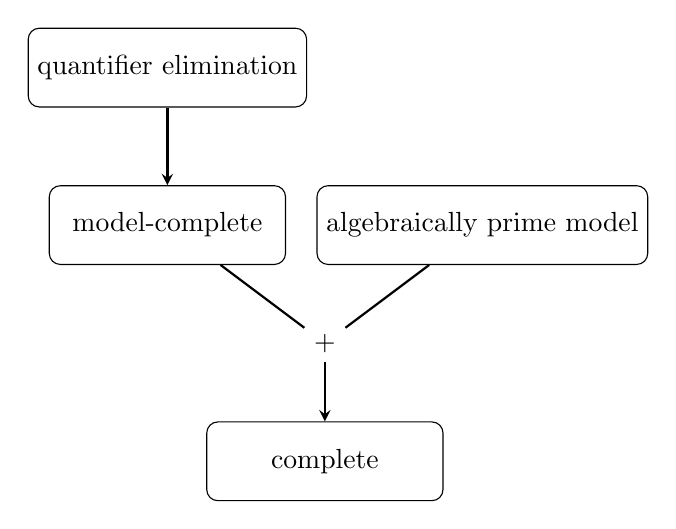
\begin{tikzpicture}
				\node[notions] (q-e) at (-2,0) {quantifier elimination};
				\node[notions] (m-c) at (-2,-2) {model-complete};
				\node[notions] (a-p-m) at (2,-2) {algebraically prime model};
				\node (cc) at (0,-3.5) {+};
				\node[notions] (c) at (0,-5) {complete};

				\draw[arrow] (q-e) -- (m-c);
				\draw[thick] (m-c) -- (cc);
				\draw[thick] (a-p-m) -- (cc);
				\draw[arrow] (cc) -- (c);
			\end{tikzpicture}
		\end{center}
	\end{tcolorbox}
\end{center}

The study of definable sets is often made quite complicated by quantifiers.

\begin{definition}
	A theory $T$ has \emph{quantifier elimination} if for every formula $\phi$ there is a quantifier-free formula $\psi$ such that
	\[
		T \models \phi \leftrightarrow \psi.
	\]
\end{definition}

\begin{definition}
	An $\mathcal{L}$-theory $T$ is \emph{strongly minimal} if for any $\mathcal{M} \models T$
	every definable subset of $M$ is either finite or cofinite.
\end{definition}

\begin{definition}
	If $T$ is a theory then $T_{\forall}$ is the set of all universal consequences of $T$.
	$\mathcal{A} \models T_{\forall}$ if and only if there is $\mathcal{M} \models T$ with $\mathcal{A} \subseteq \mathcal{M}$.

	A theory $T$ has \emph{algebraically prime models}
	if for any $\mathcal{A} \models T_{\forall}$ there is
	$\mathcal{M} \models T$ and an embedding $i:\mathcal{A} \to \mathcal{M}$
	such that for all $\mathcal{N} \models T$ and embedding $j: \mathcal{A} \to \mathcal{N}$
	there is $h: \mathcal{M} \to \mathcal{N}$ such that $j = h \circ i$.

	If $\mathcal{M}$, $\mathcal{N} \models T$ and $\mathcal{M} \subseteq \mathcal{N}$,
	$\mathcal{M}$ is \emph{simply closed} in $\mathcal{N}$ and denote
	$\mathcal{M} \prec_s \mathcal{N}$ if for any quantifier free formula
	$\phi(\overline{v},w)$ and any $\overline{a} \in M$,
	if $\mathcal{N} \models \exists w\, \phi(\overline{a},w)$,
	then so does $\mathcal{M}$.
\end{definition}

\begin{definition}
	An $\mathcal{L}$-theory $T$ is \emph{model-complete} if,
	$\mathcal{M} \prec \mathcal{N}$ whenever
	$\mathcal{M} \subseteq \mathcal{N}$  and $\mathcal{M}$, $\mathcal{N} \models T$.
\end{definition}

\begin{proposition}
	If $T$ has quantifier eliminations,
	then $T$ is model-complete.
\end{proposition}

\begin{proposition}
	Let $T$ be a model-complete theory.
	Suppose that there is $\mathcal{M}_0 \models T$ such that $\mathcal{M}_0$ embeds into every model of $T$.
	Then, $T$ is complete.
\end{proposition}

\begin{definition}
	An ordered structure $(M,<,\dots)$ is \emph{o-minimal} if
	for any definable $X \subset M$,
	there are finitely many intervals $I_1,\dots,I_m$ with endpoints in $M \cup \{\pm\infty\}$
	and a finite set $X_0$ such that $X = X_0 \cup I_1 \cup \dots \cup I_m$.
\end{definition}

\subsubsection{Algebraic Closed Fields}

% \begin{lemma}
%     $\mathbf{ACF}_{\forall}$ is the theory of integral domains.
% \end{lemma}

\begin{theorem}
	$\mathbf{ACF}$ has quantifier elimination.
\end{theorem}

\begin{corollary}
	$\mathbf{ACF}$ is model-complete and $\mathbf{ACF}_p$ is complete where $p = 0$ or $p$ is prime.
\end{corollary}

% Let $K$ be a field.
% $X \subseteq K^n$ is \emph{Zariski closed} if $X = V(S)$ for some $S \subseteq K[X_1,\dots,X_n]$.

% \begin{lemma}
%   Let $K$ be a field.
%   The subsets of $K^n$ defined by atomic formulas are exactly those of the form $V(p)$ for some $p \in K[\overline{X}]$.
%   A subset of $K^n$ is quantifier-free definable if and only if it is a Boolean combination of Zariski closed sets.
% \end{lemma}

\begin{corollary}
	Let $K$ be an algebraically closed field.
	\begin{enumerate}[label = {\roman*)}]
		\item $X \subset K^n$ is constructable if and only if it is definable.
		\item (Chevalley's Theorem) The image of a constructable set under a polynomial map is constructable.
	\end{enumerate}
\end{corollary}

\begin{corollary}
	$\mathbf{ACF}$ is a strongly minimal theory.
\end{corollary}

\subsubsection{Real Closed Fields}

\begin{definition}
	A field $F$ is \emph{orderable} if there is a linear order $<$ of $F$ making $(F,<)$ an ordered field.

	F is \emph{formally real} if $-1$ is not a sum of squares.
\end{definition}

\begin{theorem}
	If $F$ is a formally real field, then $F$ is orderable.
\end{theorem}

\begin{definition}
	A field $F$ is \emph{real closed} if it is formally real with no proper formally real algebraic extensions.
\end{definition}

\begin{theorem}
	Let $F$ be a formally real field. The following are equivalent.
	\begin{enumerate}[label = {\roman*)}]
		\item $F$ is real closed.
		\item $F(i)$ is algebraically closed.
		\item For any $a\in F$, either $a$ or $-a$ is a square and every polynomial of odd degree has a root.
	\end{enumerate}
\end{theorem}

\begin{corollary}
	The class of real closed field is an elementary class of
	$\mathcal{L}_r$-structures.
\end{corollary}

\begin{definition}
	Let $\mathbf{RCF}$ be the $\mathcal{L}_{or}$-theory axiomatized by the axioms for real closed fields
	and the axioms for ordered fields.

	If $F$ is a formally real field, a \emph{real closure} of $F$ is a real closed algebraic extension of $F$.
\end{definition}

% \begin{theorem}
%   If $(F,<)$ is an ordered field,
%   and $R_1$ and $R_2$ are real closures of $F$ where the canonical ordering extends the ordering of $F$,
%   then there is a unique field isomorphism $\phi: R_1 \to R_2$ that is identity on $F$.
% \end{theorem}

\begin{corollary}
	$\mathbf{RCF}$ has algebraically prime models.
\end{corollary}

\begin{theorem}
	The theory $\mathbf{RCF}$ admits elimination of quantifiers in $\mathcal{L}_{or}$.
\end{theorem}

\begin{corollary}
	$\mathbf{RCF}$ is complete, model complete, and decidable.
\end{corollary}

\subsection{Semialgebraic Sets and O-minimality}
\begin{definition}
	Let $F$ be an ordered field.
	$X \subset F^n$ is \emph{semialgebraic} if it is a Boolean combination of sets of the form $\{\overline{x}:p(\overline{x})>0\}$,
	where $p(\overline{X}) \in F[X_1,\dots,X_n]$.

	A function is semialgebraic if its graph is semialgebraic.
\end{definition}

\begin{corollary}[Tarski--Seidenberg Theorem]
	The semialgebraic sets are closed under projection.
\end{corollary}

\begin{corollary}
	If $F \models \mathbf{RCF}$ and $A \subseteq F^n$ is semialgebraic,
	then the closure (topological) of $F$ is semialgebraic.
\end{corollary}

\begin{definition}
	Let $F$ be a real closed field and
	$f(\overline{X}) \in F(X_1,\dots,X_n)$ be a rational function.
	$f$ is \emph{positive semi-definite} if $f(\overline{a}) \ge 0$ for all $\overline{a} \in F^n$.
\end{definition}

\begin{theorem}[Hilbert's 17th Problem]
	If $f$ is a positive semi-definite rational function over a real closed field $F$,
	then $f$ is a sum of squares of rational functions.
\end{theorem}

\begin{corollary}
	$\mathbf{RCF}$ is an o-minimal theory.
\end{corollary}

\begin{lemma}
	If $f:\mathbb{R} \to \mathbb{R}$ is semialgebraic,
	then for any open interval $U \subseteq \mathbb{R}$,
	there is a point $x\in U$ such that $f$ is continuous at $x$.
\end{lemma}

\begin{corollary}
	Let $F$ be a real closed field and $f: F \to F$ is a semialgebraic function.
	Then, one can partition $F$ into $I_1\cup \dots \cup I_m\cup X$,
	where $X$ is finite and the $I_j$ are pairwise disjoint open intervals with endpoints in $F\cup \{\pm\infty\}$
	such that $f$ is continuous on each $I_j$.
\end{corollary}

% \begin{corollary}[Curve Selection]
%   Let $F$ be a real closed field.
%   Let $X \subseteq F^n$ be semialgebraic and $\overline{a}$
%   be a point in the closure of $X$.
%   There is a continuous semialgebraic function $f:(0,r) \to F^n$
%   such that for all $\epsilon\in(0,r)$, $f(x) \in X$ and $\lim_{\epsilon\to 0} f(\epsilon) = \overline{a}$.
% \end{corollary}

\begin{corollary}
	Let $F$ be a real closed field.
	Let $E \subseteq F^n \times F^n$ be a definable equivalence relation.
	There is a definable $X \subset F^n$ such that for all
	$a \in F^n$ there is a unique $b\in X$ such that $aEb$.
	Such $X$ is called a definable \emph{transversal} of $E$.
\end{corollary}

\begin{definition}[Cell]
	Inductive definition of the collection of \emph{cells}.
	\begin{enumerate}[label = {$\bullet$}]
		\item $X \subseteq F^n$ is a $0$-cell if it is a single point.
		\item $X \subset F$ is a $1$-cell if it is an interval $(a,b)$,
		      where $a \in F \cup \{-\infty\}$, $b\in F\cup \{+\infty\}$, and $a < b$.
		\item If $X \subset F^n$ is an $n$-cell and $f: X\to F$ is a continuous definable function,
		      then $Y = \{(\overline{x},f(\overline{x})): \overline{x} \in X\}$ is an $n$-cell.
		\item Let $X \subseteq F^n$ be an $n$-cell. Suppose that $f$ is
		      either a continuous definable function from $X$ to $F$ or identically $-\infty$ and
		      $g$ is either a continuous definable function from $X$ to $F$
		      such that $f(\overline{x}) < g(\overline{x})$ for all $\overline{x} \in X$ or identically $+infty$, then
		      \[
			      Y = \{(\overline{x},y): \overline{x} \in X \land f(\overline{x}) < y < g(\overline{x})\}
		      \]
		      is an $n+1$-cell.
	\end{enumerate}
\end{definition}

% \begin{lemma}
%   Let $X \subseteq F^{n+1}$ be semialgebraic.
%   There is a natural number $N$ such that if $\overline{a}\in F^n$
%   and $X_{\overline{a}} = \{y: (\overline{a},y)\in X\}$ is finite,
%   then $|X_{\overline{a}}| < N$.
% \end{lemma}

\begin{tcolorbox}[title = {Cell Decomposition}]
	\begin{theorem}
		Let $X \subseteq F^m$ be semialgebraic.
		There are finitely many pairwise disjoint cells $C_1,\dots,C_n$ such that $X = C_1 \cup \dots \cup C_n$.
	\end{theorem}
\end{tcolorbox}

\begin{theorem}[Real Nullstellensatz]
	Let $F$ be a real closed field,
	and let $I$ be an ideal in $F[\overline{X}]$.
	Then, $V_F(I)$ is nonempty if and only if whenever $p_1,\dots,p_m\in F[\overline{X}]$ and $\sum p_i^2 \in I$,
	then all the $p_i \in I$.
\end{theorem}

Let $\mathbb{R}_{\exp} = (\mathbb{R},+,\cdot,\exp,<,0,1)$.

\begin{theorem}
	The theory of $\mathbb{R}_{\exp}$ is model-complete and o-minimal.
\end{theorem}

% \subsubsection{van den Dries's original statements}

% We work with a fixed but arbitrary o-minimal structure $(R,<,\mathcal{S})$.

% \begin{theorem}[Monotonicity Theorem]
%     Let $f: (a,b)\to R$ be a definable function on the interval $(a,b)$.
%     Then there are points $a_1 < \cdot < a_k$ in $(a,b)$ such that on each subinterval $(a_j,a_{j+1})$,
%     with $a_0 = a$, $a_{k+1} = b$,
%     the function is either constant, or strictly monotone and continuous.
% \end{theorem}

% \begin{corollary}
%     Let $f: (a,b) \to R$ be definable.
%     Then for each $c\in (a,b)$ the limit $\lim_{x\uparrow c}f(x)$
%     and $\lim_{x\downarrow c}f(x)$ exist in $R_{\infty}$.
%     Also the limits $\lim_{x\uparrow b}f(x)$ and $\lim_{x\downarrow a}f(x)$ exist in $R_{\infty}$.
% \end{corollary}

% \begin{corollary}
%     Let $f: [a,b]\to R$ be continuous and definable.
%     Then $f$ takes a maximum and a minimum value on $[a,b]$.
% \end{corollary}

% \begin{lemma}[Finiteness Lemma]
%     Let $A \subset R^2$ be definable and suppose that for each $x\in R$
%     the fiber $A_x \coloneq \{y\in R\colon (x,y)\in A\}$ is finite.
%     Then there is $N \in \mathbb{N}$ such that $A_x \le N$ for all $x\in R$.
% \end{lemma}

% A decomposition $\mathcal{D}$ of $R^m$ is said to \textbf{partition}
% a set $S \subseteq R^m$ if each cell in $\mathcal{D}$ is
% either part of $S$ or disjoint from $S$,
% in other words, if $S$ is a union of cells in $\mathcal{D}$.
% \begin{theorem}[Cell Decomposition]
%     \hfill
%     \begin{enumerate}[label = {$\mathrm{(\Roman*_{m})}$}]
%         \item Given any definable sets $A_1,dots,A_k \subset R^m$ there is a decomposition of $R^m$ partitioning each of $A_1,\dots,A_k$.
%         \item For each definable function $f: A \to R$, $A \subseteq R^m$,
%         there is a decomposition $\mathcal{D}$ of $R^m$ partitioning $A$ such that
%         the restriction $f|B: B \to R$ to each cell $B \in \mathcal{D}$ with $B \subseteq A$ is continuous.
%     \end{enumerate}
% \end{theorem}

% \begin{theorem}
%     The theory $\mathbb{R}_{\exp}$ is model-complete and o-minimal.
% \end{theorem}

% \subsubsection{}
% \begin{theorem}
%   Let $(R,<,\mathcal{S})$ be an o-minimal structure and
%   $S \subseteq R^{p+q}$ a definable set.
%   Then there is a positive integer $d = d(S)$ such that
%   for all sufficiently large $n\in\mathbb{N}$
%   each $n$-element set $F \subseteq R^q$ has at most $n^d$ subsets of the form $S_x \cap F$ with $x \in R^p$.
% \end{theorem}

% Let $\mathcal{C}$ be a collection of subsets of an infinite set $X$.
% Given $F \subseteq X$,
%   \[
%     \mathcal{C}\cap F := \{\mathcal{C}\cap F:C \in \mathcal{C}\},
%   \]
% the set of intersections of sets in $\mathcal{C}$ with $F$.
%   If $A \subseteq F$ is of the form $A = C\cap F$ for some $C\in \mathcal{C}$,
%   $A$ is \emph{cut out from $F$ by a set in $\mathcal{C}$}.
%   \[
%     f_{\mathcal{C}}(n):=\max\{|\mathcal{C}\cap F|:F\text{ is an $n$-element subset of $X$}\}.
%   \]

% \begin{theorem}
%   Either $f_{\mathcal{C}}(n) = 2^n$ for all $n$,
%   or else there is $d\in \mathbb{N}$ such that
%   $f_{\mathcal{C}}(n) = n^d$ for all sufficiently large $n$.
% \end{theorem}

% \begin{theorem}
%   Let $\mathcal{R} = (R,\dots)$ be an infinite model-theoretic structure and suppose
%   all definable relations $\Phi \subseteq R^p \times R$ for all $p > 0$, and dependent.
%   Then all definable relations $\Phi \subseteq R^p \times R^q$,
%   for all $p$, $q > 0$, are dependent.
% \end{theorem}

% \begin{theorem}[Ramsey's Theorem]
%   Given positive integers $M$, $r$ and $k$,
%   there is a positive integer $N = N(M,r,k)$ so large that
%   if $X$ is a set with $|X| \ge N$ and
%   $X^{(r)} = P_1 \cup P_2 \cup \dots \cup P_k$,
%   then there is a set $Y \subseteq X$ with $|Y|=M$ such that
%   $Y^{(r)} \subseteq P_j$ for some $j\in \{1,\dots,k\}$.
% \end{theorem}

% \begin{definition}
%   Let $X$ be an infinite set.
%   Given a relation $A \subseteq X^r$,
%   a finite sequence $x_1,\dots,x_M$ in $X$ is \emph{$A$-indiscernible} if
%   \[
%     (x_{i(1)},\dots,x_{i(r)})\in A \iff (x_{j(1)},\dots,x_{j(r)}) \in A.
%   \]
%   whenever $1\le i(1) < \cdots < i(r) \le M$ and
%   $1\le j(1) < \cdots < j(r) \le M$.
%   Let $\mathcal{A}$ be a collection of relations on $X$,
%   that is, each element of $\mathcal{A}$ is a set $A \subseteq A^r$,
%   with $r \in\mathbb{N}$ depending on $A$.
%   Then a sequence $x_1,\dots,x_M$ in $X$ is called \emph{$\mathcal{A}$-indiscernible} if it is $A$-indiscernible for each $A \in \mathcal{A}$.
%   A \emph{subsequence} of a sequence $x_1,\dots,x_N$ is by definition a sequence $x_{i(1)},\dots,x_{i(M)}$ with
%   $1\le i(1)< \dots < i(M) \le N$.
% \end{definition}

% \begin{corollary}
%     Let $X$ be an infinite set and $\mathcal{A}$ a finite collection of relation on $X$.
%     Then, given any positive integer $M$ there is a positive integer $N$ so large that each sequence in $X$ of length $N$ contains an $\mathcal{A}$-indiscernible subsequence of length $M$.
% \end{corollary}

% TODO

% \subsubsection{}
% Fix an o-minimal expansion $(R,<,\mathcal{S})$ of an ordered abelian group $(R,<,0,-,+)$.

% Definable curves play a role similar to that of sequences in $\mathbb{R}$, better properties.

% \begin{corollary}[Curve Selection]
%     If $a\in\mathrm{cl}(X)-X$,
%     where $X$ is definable,
%     then there is a definable continuous injective map
%     $\gamma: (0,\epsilon) \to X$, for some $\epsilon > 0$,
%     such that $\lim_{t\to 0}\gamma(t) = a$.
% \end{corollary}

% \begin{lemma}
%     Let $f: X \to R^n$ be a definable continuous map on a closed bounded set $X \subseteq R^m$.
%     Then $f(X)$ is bounded in $R^n$.
% \end{lemma}

% \begin{proposition}
%     If $f: X \to R^n$ is a continuous definable map on a closed bounded set $X \subseteq R^m$,
%     then $f(X)$ is closed and bounded in $R^m$.
% \end{proposition}

% TODO

% \subsubsection{}
% \begin{theorem}[Triangulation Theorem]
%     Let $S \subset R^m$ be a definable set,
%     with definable subsets $S_1,\dots,S_k$.
%     Then $S$ has a triangulation in $R^m$ that is compatible with these subsets.
% \end{theorem}

% TODO

\subsection{About Types}
Suppose that $\mathcal{M}$ is an $\mathcal{L}$-structure and $A \subseteq M$.
Let $\mathcal{L}_A$ be the language obtained by adding to $\mathcal{L}$ constant symbols for each $a\in A$.
We can naturally view $\mathcal{M}$ as an $\mathcal{L}_A$-structure by interpreting the new symbols in the obvious way.
Let $\mathrm{Th}_A(\mathcal{M})$ be the set of all $\mathcal{L}_A$-sentences true in $\mathcal{M}$.
% Note that $\mathrm{Th}_A(\mathcal{M}) \subseteq \mathrm{Diag_el}(\mathcal{M})$.

\begin{definition}
	Let $p$ be the set of $\mathcal{L}_A$-formulas in free variables $v_1,\dots,v_n$.
	$p$ is an \emph{$n$-type} if $p\cup \mathrm{Th}_A(\mathcal{M})$ is satisfiable.
	$p$ is a \emph{complete $n$-type} if $\phi\in p$ or $\neg\phi\in p$ for all $\mathcal{L}_A$-formulas $\phi$ with free variables from $v_1,\dots,v_n$.
	Let $S^{\mathcal{M}}_n(A)$ be the set of all complete $n$-types.

	Incomplete types are referred to as \emph{partial types}.
	We often write $p(v_1,\dots,v_n)$ to stress that $p$ is an $n$-type.

	If $\mathcal{M}$ is any $\mathcal{L}$-structure,
	$A \subset M$, and $(a_1,\dots,a_n)\in M^n$,
	let $\mathrm{tp}^{\mathcal{M}}(\overline{a}/A) = \{\phi(v_1,\dots,v_m)\in \mathcal{L}_A:\mathcal{M}\models \phi(a_1,\dots,a_n)\}$.
	Then, $\mathrm{tp}^{\mathcal{M}}(\overline{a}/A)$ is a complete $n$-type.
	Write $\mathrm{tp}^{\mathcal{M}}(\overline{a})$ for $\mathrm{tp}^{\mathcal{M}}(\overline{a}/\emptyset)$.

	If $p$ is an $n$-type over $A$,
	$\overline{a}\in M^n$ \emph{realizes $p$} if $\mathcal{M} \models \phi(\overline{a})$ for all $\phi\in p$.
	If $p$ is not realized in $\mathcal{M}$,
	then $\mathcal{M}$ \emph{omits $p$}.
\end{definition}

\begin{definition}
	Let $T$ be a complete theory in a countable language,
	and let $\kappa$ be an infinite cardinal.
	$T$ is \emph{$\kappa$-stable} if whenever $\mathcal{M}\models T$,
	$A \subseteq M$, and $|A| = \kappa$, then $|S^{\mathcal{M}}_n(A)| = \kappa$.
\end{definition}

\begin{definition}
	Let $\phi(v_1,\dots,v_n)$ be an $\mathcal{L}$-formula such that $T \cup \{\phi(\overline{v})\}$ is satisfiable,
	and let $p$ be an $n$-type.
	\emph{$\phi$ isolates $p$} if
	\[
		T \models \forall\overline{v}(\phi(\overline{v}) \to \psi(\overline{v}))
	\]
	for all $\psi \in p$.
\end{definition}
Note that if $p$ is a complete type and $\phi(\overline{v})$ isolates $p$, then
\[
	T \models \phi(\overline{v}) \to \psi(\overline{{v}}) \iff \psi(\overline{v})\in p
\]
for all formulas $\psi(\overline{v})$.
In particular, for all formulas $\psi(\overline{v})$,
exactly one of $T + \phi(\overline{v}) \land \psi(\overline{v})$ and $T + \phi(\overline{v}) \land \neg\psi(\overline{v})$ is satisfiable.

\begin{theorem}[Omitting Types Theorem]
	Let $\mathcal{L}$ be a countable language,
	$T$ an $\mathcal{L}$-theory,
	and $p$ a (possibly incomplete) non-isolated $n$-type over $\emptyset$.
	Then, there is a countable $\mathcal{M} \models T$ omitting $p$.
\end{theorem}

\begin{definition}
	$\mathcal{M}\models T$ is a \emph{prime model} of $T$ if whenever $\mathcal{N}\models T$ there is an elementary embedding of $\mathcal{M}$ into $\mathcal{N}$.
\end{definition}

\begin{definition}
	$\mathcal{M}\models T$ is \emph{atomic} if $\mathrm{tp}^{\mathcal{M}}(\overline{a})$ is isolated for all $\overline{a} \in M^n$.
\end{definition}

\begin{definition}
	Let $\kappa$ be an infinite cardinal.
	$\mathcal{M}\models T$ is \emph{$\kappa$-homogeneous}
	if whenever $A \subset M$ with $|A| < \kappa$,
	$f: A \to M$ is a partial elementary map,
	and $a \in M$, there is $f^*\supseteq f$ such that $f^*: A\cup \{a\} \to M$ is partial elementary.

	$\mathcal{M}$ is \emph{homogeneous} if it is $|M|$-homogeneous.
\end{definition}

\begin{definition}
	Let $T$ be a complete theory in a countable language,
	and let $\kappa$ be an infinite cardinal.
	$T$ is \emph{$\kappa$-stable} if whenever $\mathcal{M}\models T$,
	$A \subseteq M$, and $|A| = \kappa$, then $|S^{\mathcal{M}}_n(A)| = \kappa$.

	$\mathcal{M}$ is $\kappa$-stable if $\mathrm{Th}(\mathcal{M})$ is $\kappa$-stable.
\end{definition}

\begin{definition}
	Let $\kappa$ be an infinite cardinal.
	$\mathcal{M} \models T$ is $\kappa$-saturated if,
	for all $A \subseteq M$, if $|A| < \kappa$ and $p \in S^{\mathcal{M}}_n(A)$,
	then $p$ is realized in $\mathcal{M}$.

	$\mathcal{M}$ is \emph{saturated} if it is $|M|$-saturated.
\end{definition}

\begin{proposition}
	If $\mathcal{M}$ is $\kappa$-saturated,
	then $\mathcal{M}$ is $\kappa$-homogeneous.
\end{proposition}

\begin{definition}
	$\mathcal{M} \models T$ is \emph{$\kappa$-universal} if for all $\mathcal{N}\models T$ with $|N| < \kappa$ there is an elementary embedding of $\mathcal{N}$ into $\mathcal{M}$.

	$\mathcal{M}$ is \emph{universal} if it is $|M|^+$-universal.
\end{definition}

\begin{theorem}
	Let $\kappa \ge \aleph_0$.
	The following are equivalent.
	\begin{enumerate}[label = {\roman*)}]
		\item $\mathcal{M}$ is $\kappa$-saturated.
		\item $\mathcal{M}$ is $\kappa$-homogeneous and $\kappa^+$-universal.
	\end{enumerate}
	If $\kappa \ge \aleph_1$, i) and ii) are also equivalent to:
	\begin{enumerate}[resume, label = {\roman*)}]
		\item $\mathcal{M}$ is $\kappa$-homogeneous and $\kappa$-universal.
	\end{enumerate}
\end{theorem}

\begin{corollary}
	$\mathcal{M}$ is saturated if and only if it is homogeneous and universal.
\end{corollary}

\begin{theorem}
	If $\mathcal{M}$ and $\mathcal{N}$ are saturated models of $T$ of cardinality of $\kappa$,
	then $\mathcal{M}\cong\mathcal{N}$.
\end{theorem}

\begin{proposition}
	Let $\mathcal{M}$ be saturated.
	Let $A \subset M$ with $|A| < |M|$.
	Let $X \subset M^n$ be definable with parameters from $M$.
	Then, $X$ is $A$-definable if and only if every automorphism of $\mathcal{M}$ that fixes $A$ pointwise fixes the $X$ setwise.
\end{proposition}

$b \in M$ is \emph{definable from $A$} if $\{b\}$ is $A$-definable.
\begin{corollary}
	Let $\mathcal{M}$ be saturated,
	and let $A \subset M$ with $|A| < |M|$.
	Then, $b$ is definable from $A$ if and only if $b$ is fixed by all automorphisms of $\mathcal{M}$ that fix $A$ pointwise.
\end{corollary}

$b$ is \emph{algebraic} over $A$ if there is a finite $A$-definable set $X$ such that $b\in X$.
\begin{proposition}
	Let $\mathcal{M}$ be saturated.
	Let $A \subset M$ with $|A| < |M|$ and $b \in M$.
	The following are equivalent:
	\begin{enumerate}[label = {\roman*)}]
		\item $b$ is algebraic over $A$;
		\item $b$ has only finitely many images under automorphisms of $\mathcal{M}$ fixing $A$ pointwise;
		\item $\mathrm{tp}^{\mathcal{M}}(b/A)$ has finitely many realization.
	\end{enumerate}
\end{proposition}

\subsection{Definable Spaces and Quotients}
\subsubsection{Definable spaces}
Let a covering $S = \bigcup_i U_i$ of a set $S$ by subsets $U_i$ ($i\in I$) be given,
and for each index $i \in I$ a set-theoretic bijection $g_i: U_i \to U'_i$ a topological space,
such that the transition maps are continuous.

Suppose that the index set $I$ is finite,
that each $U'_i \subseteq R^{m(i)}$ is a definable set,
and for each pair $i$, $j$ the set $g_i(U_i\cap U_j) \subseteq U'_i$
is definable and $g_{ij}: g_i(U_i\cap U_j) \to g_j(U_j\cap U_i)$ is definable.
(Such a family is called a \emph{definable atlas of $S$}.)

Let $X \subseteq S$ and $f : X \to R$;
call $X$ \emph{definable} if $g_i(X\cup U_i) \subseteq I'_i$ is definable for each $i$,
and call $f$ \emph{definable} if $X$ is definable and
$f_i : g_i(X \cap U_i) \to R$ given by $f_i(x) = f(g_i^{-1}(x))$ is definable for each $i$.
If $X = X_1\cup \cdots \cup X_n$,
where all $X_k$ are definable,
then a function $f: X \to R$ is definable if and only if each restriction $f|X_k: X_k \to R$ is definable.

Note that $U_i$ is definable,
and for $g_i = (g_{i1},\dots,g_{im(i)}) : U_i \to R^{m(i)}$,
each $g_{ik}$ is definable.
Let $\mathbf{DO}(S)$ be the collection of definable open subsets of $S$,
and for each $U \in \mathbf{DO}(S)$,
let $\mathbf{DC}(U)$ be the $R$-algebra of definable continuous functions $f: U \to R$.
Then we call the set $S$ equipped with the sheaf $(\mathbf{DC}(U))_{U \in \mathbf{DO}(S)}$ a \emph{definable space}.

\begin{definition}
	Let $S$ and $T$ be definable spaces.
	Then a map $F: S \to T$ is said to be \emph{definable} if its graph $\Gamma(F)$ is a definable subset of
	the product space $S \times T$.
\end{definition}

\begin{definition}
	Recall that a topological space $S$ is said to be regular if for each $a \in  S$ and
	open $U \subseteq S$ with $a \in U$ there is an open $V \subseteq S$ with $a \in V$ and $\mathrm{cl}(V) \subseteq U$.
	A definable space $S$ is regular if and only if for each $a \in S$ and definable open $U \subseteq S$ with $a \in U$
	there is a definable open $V \subseteq S$ with $a \in V$ and $\mathrm{cl}(V) \subseteq U$,
	and also if and only if for each $a \in S$ and definable closed $X \subseteq S$ with $a \notin X$
	there are disjoint definable open neighborhoods of $a$ and $X$ in $S$.
\end{definition}

\subsubsection{Definable quotient spaces}

Let $E \subseteq X\times X$ be a definable equivalence relation on a definable set $X \subseteq R^m$.

\begin{definition}
	A \emph{definable quotient of $X$ be $E$} is a pair $(p,Y)$ consisting of a definable set $Y \subseteq R^n$ and definable continuous surjective map $p: X\to Y$ such that
	\begin{enumerate}[label = {(\roman*)}]
		\item $E = E_p$, i.e., $(x_1,x_2) \in E \iff p(x_1) = p(x_2)$ for all $x_1$, $x_2 \in X$;
		\item $p$ is definably identifying, i.e., for all definable $K \subseteq Y$, if $p^{-1}(K)$ is closed in $X$, then $K$ is closed in $Y$.
	\end{enumerate}
\end{definition}

Let $E$ be a definable equivalence relation on a definable set $X$.
Let $pr_1 : E \to X$ and $pr_2 : E \to X$ be the restrictions of the two projection maps $X\times X \to X$.

$E$ is called \emph{definably proper over $X$} if $pr_1$ is a definably proper map.

\begin{theorem}
	Suppose the definable equivalence relation $E$ on the definable set $X$ is definably proper over $X$.
	Then $X/E$ exists as a definably proper quotient of $X$.
\end{theorem}

\section{Definable complex geometry}
Materials follow from \cite{MR2441378}.

Let $\mathbf{R}$ be a real closed field and $\mathbf{K}$ its algebraic closure,
identified with $\mathbf{R}^2$ (after fixing a square-root of $-1$).

\subsection{Topological aspects}

\begin{definition}
	A \emph{definable $C^0$ $\mathbf{R}$-manifold of dimension $n$, with respect to $\mathbf{R}$} is a set $X$,
	covered by finitely many nonempty sets $U_1, \dots, U_k$,
	and for each $i = 1, \dots, k$,
	there is a set-theoretic bijection $\phi_i:U_i \to V_i$,
	where $V_i$ is definable and open in $\mathbf{R}^n$ and such that each $\phi_i(U_j\cap U_i)$ is definable an open
	and the transition maps are definable and continuous.
	Moreover, the topology induced on $X$ by this covering is Hausdorff.

	A manifold is a \emph{$C^p$ $\mathbf{R}$-manifold} if in addition
	the transition maps are $C^p$ with respect to the field $\mathbf{R}$.
\end{definition}

\begin{definition}
	Let $X$ be a definable subset of $\mathbf{R}^n$.
	$X$ is called \emph{definably compact} if for every definable continuous $\gamma:(0,1) \to X$ the limit of $\gamma(t)$,
	as $t$ tends to $0$ in $\mathbf{R}$, exists in $X$.
	This is equivalent to $X$ being closed and bounded in $\mathbf{R}^n$.

	A definable set $X \subseteq \mathbf{R}^n$ is \emph{locally definably compact}
	if every $x \in $ has a definable neighborhood $V\subseteq X$
	(i.e., $V$ contains an $X$-open set around $x$)
	which is definably compact.

	$X \subseteq \mathbf{R}^n$ is \emph{locally closed} if there is a (definable) open set $U \subseteq \mathbf{R}^n$ containing $X$
	such that $X$ is relatively closed in $U$.

	Let $U$ be an open subset of $\mathbf{R}^n$.
	For $X \subseteq U$,
	the \emph{frontier of $X$ in $U$} is defined as $Fr_U(X) = Cl_U(X)\backslash X$,
	where $Cl_U(X)$ is the closure of $X$ in $U$.
	If $U = \mathbf{R}^n$ then we write $Fr(X)$ instead of $Fr_{\mathbf{R}^n}$.
\end{definition}

\begin{lemma}
	Let $X$ be a definable subset of $\mathbf{R}^n$.
	Then the following are equivalent:
	\begin{enumerate}[label = {(\roman*)}]
		\item $X$ is locally definably compact.
		\item $X$ is locally closed in $\mathbf{R}^n$.
		\item $Fr(X)$ is closed subset of $\mathbf{R}^n$.
	\end{enumerate}
\end{lemma}

\begin{definition}
	Let $f$ be a definable continuous map from a definable $X \subseteq \mathbf{R}^n$ into $Y \subseteq \mathbf{R}^k$.

	For $b \in Y$, $f$ is \emph{definably proper over $b$} if for every definable curve $\gamma:(0,1) \to X$ such that $\lim_{t\to 0} f(\gamma(t)) = b$,
	$\gamma(t)$ tends to some limit in $X$ as $t$ tends to $0$.
	If $f: X \to Y$ is definably proper over every $b\in Y$ then
	we say that $f$ is \emph{definably proper over $Y$} or just
	$f$ is \emph{definably proper}.

	For $A \subseteq X$, we say that $f|A$ is \emph{definably proper over its image} if $f|A : A \to f(A)$ is definably proper over $f(A)$.

	We say that $f$ is \emph{bounded over $b\in Y$} if there is a neighborhood $W \subseteq Y$ of $b$ such that $f^{-1}(W)$ is bounded subset of $\mathbf{R}^n$.
\end{definition}

% \begin{lemma}
%   For $f: X \to Y$ a definable continuous map,
%   $X \subseteq \mathbf{R}^n$,
%   and $y\in Y$, the following are equivalent:
%   \begin{enumerate}[label = {(\roman*)}]
%     \item $f$ is definably proper over $y$.
%     \item $f$ is bounded over $y$ and the intersection of the closure of the graph of $f$
%       in $\mathbf{R}^n\times Y$ with $Fr(X)\times \{y\}$ is empty.
%   \end{enumerate}
% \end{lemma}

% \begin{lemma}
%   Let $X \subseteq \mathbf{R}^n$ be a definable,
%   locally closed set, $f: X \to \mathbf{R}^k$ a definable
%   continuous map. Then,
%   \begin{enumerate}[label = {(\roman*)}]
%     \item The set of all $y \in \mathbf{R}^k$ such that $f$ is definably proper over $y$ is open in $\mathbf{R}^k$.
%     \item If $f$ is definably proper over $f(X)$, then $f(X)$ is locally closed set.
%   \end{enumerate}
% \end{lemma}

Assume that the structure is $\omega_1$-saturated if generic points are mentioned.

\begin{definition}
	Let $H \subseteq \mathbf{K}^n$ be a $d$-dimensional $\mathbf{K}$-subspace of $\mathbf{K}^n$.
	$H$ is \emph{generic over a set $C \subseteq \mathbf{R}$} if the following holds:
	Let $\{H_s: s \in S\}$ be some $C$-definable parametrization of all $d$-dimensional $\mathbf{K}$-linear subspaces of $\mathbf{K}^n$.
	Then $H = H_s$ for some $s$ generic in $S$ over $C$.
\end{definition}

For $H$ a $d$-dimensional $\mathbf{K}$-subspace of $\mathbf{K}^n$,
an orthogonal projection $\pi:\mathbf{K}^n \to H$ is \emph{generic over $C$} if $H$ is generic over $C$.

\begin{definition}
	A definable subset $A$ of $\mathbf{R}^k$ is called an $m$-dimensional $C^p$ $\mathbf{R}$-submanifold of $\mathbf{R}^k$
	if for every $x\in A$ there is a definable open neighborhood $U$ of $x$ and definable $C^p$ (with respect to $\mathbf{R}$) map
	$f: U \to \mathbf{R}^{n-m}$ such that $A \cap U = f^{-1}(0)$ and the rank of the $\mathbf{R}$-differential $df_x$ of $f$ at $x$ equals $n-m$.
\end{definition}

In classical complex analytic geometry,
given a complex analytic set $A$ and $p \in A$,
one moves to a local coordinates system,
chosen properly, in order to ensure that the projection map from $A$ onto (some of) the coordinates is a proper map in this neighborhood.
The following theorem is probably the most significant advantage of the o-minimal setting in comparison with the general classical setting.
It allows us to work “globally” rather than “locally”.

\begin{tcolorbox}[title = {The main covering theorem}]
	\begin{theorem}
		Let $A$ be a definable, locally closed subset of $\mathbf{K}^n$,
		such that $\dim_{\mathbf{R}}A = 2d < 2n$.

		Then there are definable open sets $U_1,\dots,U_k \subseteq \mathbf{K}^n$ and $d$-dimensional $\mathbf{K}$-linear subspaces $L_1,\dots,L_k$ such that
		\begin{enumerate}[label = {(\arabic*)}]
			\item $\bigcup_{i=1}^k U_i = \mathbf{K}^n\backslash Fr_{\mathbf{K}^n}(A)$ (in partition $A$ is contained in the union of the $U_i$'s).
			\item For each $i = 1,\dots,k$, if $\pi_i:\mathbf{K}^n \to L_i$ is the orthogonal projection, then $\pi_i|U_i\cap A$ is definably proper over $\pi_i(U_i)$.
			\item If furthermore $A$ is a $C^1$ $\mathbf{R}$-submanifold of $\mathbf{K}^n$ then the $U_i$'s and $L_i$'s can be chosen to satisfy also:
			      For every $i=1,\dots,k$ the map $\pi_1|A\cap U_i$ is local diffeomorphism and there is $m = m_i$ such that every $y \in \pi_i(U_i)$ has exactly $m$ pre-images under $\pi_i$ in $A \cap U_i$.
		\end{enumerate}
	\end{theorem}
\end{tcolorbox}

\subsection{Analytic aspects}
For $U \subseteq \mathbf{K}$ a definable open set and $z_0 \in U$,
a definable function $f: U \to \mathbf{K}$ is \emph{$\mathbf{K}$-differentiable at $z_0$} if $\lim_{h\to 0}(f(z_0+h) - f(z_0))/h$ exists in $\mathbf{K}$.
If $f$ is $\mathbf{K}$-differentiable at every point on $U$ then
$f$ is \emph{$\mathbf{K}$-holomorphic in $U$}.

\begin{definition}
	A \emph{$d$-dimensional $\mathbf{K}$-manifold} is a set $X$,
	together with a finite cover $X = \bigcup_{i=1}^r U_i$,
	and for each $i = 1,\dots,r$ a set-theoretic bijection $\phi_i: U_i \to V_i$,
	with $V_i$ a definable subset open of $\mathbf{K}^d$,
	such that for each $i$, $j$,
	the set $\phi_i(U_i \cap U_j)$ is a definable open subset of $V_i$ and the transition maps $\phi_j \phi_i^{-1}$ are $\mathbf{K}$-holomorphic.
	Moreover, the naturally induced topology is Hausdorff.
\end{definition}

\begin{definition}
	Let $N$ be a $\mathbf{K}$-manifold.
	A definable $M \subseteq N$ is called a \emph{$d$-dimensional $\mathbf{K}$-submanifold of $N$} if for every $a\in M$ there is a definable open set $U \subseteq N$ containing $a$ and a $\mathbf{K}$-holomorphic $f: U \to \mathbf{K}^{n-d}$ such that $M \cup U = f^{-1}(0)$ and $\mathrm{rank}_{\mathbf{K}}(Df_a) = n-d$,
	where $Df_x$ is the $\mathbf{K}$-differential of $f$ at $x$.
\end{definition}

\begin{definition}
	If $A$ is a definable subset of a $\mathbf{K}$-manifold $M$,
	then $A$ is a \emph{locally $\mathbf{K}$-analytic subset} of $M$
	if for every $a\in A$ there is a definable open $V \subseteq M$ containing $a$ and a $\mathbf{K}$-holomorphic map $f : V \to \mathbf{K}^m$,
	for some $m$, such that $A\cap V= f^{-1}(0)$.
	A is called a \emph{$\mathbf{K}$-analytic subset} of $M$ if in addition to the above $A$ is closed in $M$.

	A definable closed $A \subseteq M$ is \emph{finitely $\mathbf{K}$-analytic subset} of $M$ if it can be covered by finitely many definable open subsets of $M$,
	on each of which $A$ is the zero set of some $\mathbf{K}$-holomorphic map.
	A $\mathbf{K}$-analytic subset $A $of $M$ is called \emph{reducible} if it can be written as $A= A_1 \cup A_2$,
	where $A_1$ and $A_2$ are $\mathbf{K}$-analytic in $M$ and none of the $A_i$'s is contained in the other.
	When $A$ is not reducible it is called \emph{irreducible}.
\end{definition}

\begin{theorem}
	Let $G \subseteq \mathbb{C}^n$ be an open set and let $X$ be a $\mathbb{C}$-analytic subset of $G$ such that both $X$ and $G$ are definable in $\mathbb{R}_{\exp}$.
	Then there is a complex algebraic set $A \subseteq \mathbb{C}^n$ such that $X$ is the union of several irreducible components of $A\cap G$.
\end{theorem}

\begin{definition}
	Let $N$ be a $\mathbf{K}$-manifold.
	If $A \subseteq N$ is an arbitrary definable set then $\mathrm{Reg}_{\mathbf{K}}A$ is the set of all points $z \in A$ such that in some neighborhood of $a$,
	the set $A$ is a $\mathbf{K}$-submanifold of $N$.
	We let $\mathrm{Sing}_{\mathbf{K}}A = A \backslash \mathrm{Reg}_{\mathbf{K}}A$.
\end{definition}

\begin{lemma}
	If $A$ is a $\mathbf{K}$-analytic subset of a $\mathbf{K}$-manifold $N$ and $\mathrm{Reg}_{\mathbf{K}}A$ is definably connected then $A$ is irreducible.
	In particular, the number of irreducible components of $A$ is finite.
\end{lemma}

\begin{lemma}
	Let $U$ be a definable open subset of $\mathbf{K}^n$,
	$A$ a definable relatively closed subset of $U$
	whose $\mathbf{R}$-dimension is $2d$.
	Assume that $\mathrm{Reg}_{\mathbf{K}}A$ is definably connected,
	dense in $A$, and that $\dim_{\mathbf{R}}(\mathrm{Sing}_{\mathbf{K}}A) \le 2d-2$.
	Assume also that the projection map onto the first $d$ coordinates,
	$\pi : A \to \mathbf{K}^d$,
	is finite-to-one and definably proper over its image.

	Then, $\pi(A)$ is open in $\mathbf{K}^d$ and there is an $r\in \mathbb{N}$ and a $\mathbf{K}$-holomorphic map
	$\Psi: \pi(A) \times \mathbf{K}^{n-d} \to \mathbf{K}^d$ such that $A$ is the zero set of $\Psi$.

	Moreover, the map $\Psi$ can be definably recovered in the structure $(\mathbf{R},<,+,\cdot,A)$.
\end{lemma}

\begin{tcolorbox}
	\begin{theorem}
		Let $M$ ba $\mathbf{K}$-manifold and $A$ a definable closed subset of $M$.
		Assume that for every open $U \subseteq M$,
		$\dim_{\mathbf{R}}(\mathrm{Sing}_{\mathbf{K}}(A\cap U)) \le \dim_{\mathbf{R}}(A\cap U) -2$.
		Then $A$ is a finitely $\mathbf{K}$-analytic subset of $M$.

		In particular, every $\mathbf{K}$-analytic subset of $M$ is finitely $\mathbf{K}$-analytic.
	\end{theorem}
\end{tcolorbox}

\begin{corollary}
	If $M$ is a $\mathbf{K}$-manifold and $A$ a closed definable subset of $M$ then the following are equivalent:
	\begin{enumerate}[label = (\roman*)]
		\item For every open $W \subseteq \mathbf{K}^n$, $\dim_{\mathbf{R}}(\mathrm{Sing}_{\mathbf{K}}(A\cap W)) \le \dim_{\mathbf{R}}(A\cap W) -2$.
		\item $A$ is $\mathbf{K}$-analytic subset of $M$.
		\item $A$ is finitely $\mathbf{K}$-analytic subset of $M$.
	\end{enumerate}
	Moreover, in (iii) the open sets and $\mathbf{K}$-holomorphic functions which carve $A$ in each of them can be chosen be definable in the structure $(R,<,+,\cdot,A)$.
\end{corollary}

\begin{tcolorbox}[title = {Definable Chow's Theorem}]
	\begin{theorem}
		Let $A$ be a definable $\mathbf{K}$-algebraic subset of $\mathbf{K}^n$.
		Then $A$ is an algebraic set over $\mathbf{K}$.
	\end{theorem}
\end{tcolorbox}

\begin{corollary}
	Every bounded $\mathbf{K}$-analytic subset of $\mathbf{K}^n$ is finite.
\end{corollary}

\begin{tcolorbox}
	\begin{theorem}
		Let $M$ be a $\mathbf{K}$-manifold and let $A$ be a $\mathbf{K}$-analytic subset of $M$.
		Then $\mathrm{Sing}_{\mathbf{K}}(A)$ is a $\mathbf{K}$-analytic subset of $M$.
	\end{theorem}
\end{tcolorbox}

\begin{theorem}
	Assume that $A \subseteq U \subseteq \mathbf{K}^n$ is a $\mathbf{K}$-analytic set and $f: U \to \mathbf{K}^d$ is $\mathbf{K}$-holomorphic.
	Then the map $x\mapsto \dim_{\mathbf{K}}(A\cap f^{-1}(f(x)))_x$ is upper semi-continuous on $A$.
\end{theorem}

\begin{theorem}[The Dimension Theorem]
	Let $M$ be an $n$-dimensional \hspace{0em}
	$\mathbf{K}$-manifold,
	$X$, $Y$ definable, irreducible $\mathbf{K}$-analytic subsets of $M$.
	Then every irreducible component of $X \cap Y$ has $\mathbf{K}$-dimension not less than $\dim_{\mathbf{K}}X + \dim_{\mathbf{K}}Y - n$.
\end{theorem}

\begin{theorem}[Remmert's Proper Mapping Theorem]
	Let $f: M \to N$ be a $\mathbf{K}$-holomorphic map between $\mathbf{K}$-manifolds.
	Let $A \subseteq M$ be a $\mathbf{K}$-analytic subset.
	Assume that $f(A)$ is a closed subset of $N$.
	Then $f(A)$ is a $\mathbf{K}$-analytic subset of $N$.
\end{theorem}

\subsubsection{Zariski structures}

Classical complex manifold version:
\begin{theorem}[{\cite{zbMATH00554994}}]
	Consider the structure whose universe is a compact complex manifold,
	and whose atomic relations are all the complex analytic subsets of $M$ and of its Cartesian products.
	Then the structure eliminates quantifiers,
	it is stable of finite Morley Rank and moreover,
	it is a Zariski structure
	(with the closed sets taken as the K-analytic ones).
\end{theorem}

Model theoretic version:
\begin{theorem}
	Let $M$ be a definably compact $\mathbf{K}$-manifold,
	equipped with all $\mathbf{K}$-analytic subsets of Cartesian products of $M$.
	Then $M$ eliminates quantifiers,
	it is stable of finite Morley rank and a (complete) Zariski structure
	(with the closed sets taken as the $\mathbf{K}$-analytic ones).
\end{theorem}

\subsection{Applications}
\subsubsection{Meromorphic}
Let $M$, $N$ be $\mathbf{K}$-manifolds,
$U$ a definable open subset of $M$
whose complement is a $\mathbf{K}$-analytic subset of $M$.
A $\mathbf{K}$-holomorphic map $f: U \to N$ is
\emph{$\mathbf{K}$-meromorphic} if the closure of its graph in $M \times N$
is a $\mathbf{K}$-analytic subset of $M \times N$.

\begin{corollary}
	Let $M$, $N$ be $\mathbf{K}$-manifolds,
	$S \subseteq M$ an irreducible $\mathbf{K}$-analytic subset of $M$,
	and assume that $L$ is a closed definable subset of $S$ which contains $\mathrm{Sing}_{\mathbf{K}}S$.
	If $f: S \backslash L \to N$ is a $\mathbf{K}$-holomorphic map and
	$\dim_{\mathbf{R}}L \ge \dim_{\mathbf{R}}S -2$ then
	the closure of the graph of $f$ in $M \times N$ is a $\mathbf{K}$-analytic subset of $M \times N$.
\end{corollary}

\subsubsection{Campana--Fujiki}
\begin{definition}
	Let $M$ be a $\mathbf{K}$-manifold,
	a \emph{$\mathbf{K}$-holomorphic-vector-bundle over $M$,
		of dimension $d$} consists of a $\mathbf{K}$-manifold,
	a $\mathbf{K}$-holomorphic map $\rho: X \to M$,
	such that :

	There is finite cover of $M$ by definable open sets $M = \bigcup_{i=1}^k V_i$,
	and for each $i = 1,\dots,k$ there is a $\mathbf{K}$-biholomorphism
	$\phi_i: V \times \mathbf{K}^d \to \rho^{-1}(V_i)$ such that $\rho\phi_i(x,y) = x$.
	Furthermore, if $x \in V_i\cap V_j \neq\emptyset$ then $\phi_i^{-1}\phi_j$ induces
	a $\mathbf{K}$-linear automorphism $g_{i,j}(x)$ of the vector space $\mathbf{K}^d$,
	in the fiber above $x$.
	The map $x\mapsto g_{i,j}(x)$ is $\mathbf{K}$-holomorphic from $V_i\cap V_j$ into $\mathrm{GL}(d_i,\mathbf{K})$.
\end{definition}

\begin{tcolorbox}
	\begin{theorem}
		Assume that $N$, $M$ are $\mathbf{K}$-manifolds,
		and $S$ is an irreducible $\mathbf{K}$-analytic subset of $N \times M$.
		Then there is a $\mathbf{K}$-holomorphic vector-bundle
		$\pi: V \to M$, a $\mathbf{K}$-meromorphic map $\sigma: S \to \mathbb{P}(V)$,
		and a Zariski open subset $S^0$ of $S$ such that for all
		$(b,a)$, $(b',a)\in S^0$, $\sigma(b,a) = \sigma(b',a)$ if and only if
		$S_b = S_{b'}$ near $a$, and the following diagram of $\mathbf{K}$-meromorphic
		maps is commutative
		\[
			\begin{tikzcd}
				S^0 \ar[rr,"\sigma"]\ar[dr,"\pi_M"'] & & \mathbb{P}(V)\ar[dl,"\pi"] \\
				& M &
			\end{tikzcd}
		\]
	\end{theorem}
\end{tcolorbox}

\subsubsection{Fnite version of the Coherence Theorem}

Let $M$ be a $\mathbf{K}$-manifold of dimension $n$.
For $U \subseteq M$ a definable open set,
let $\mathcal{O}(U)$ denote the ring of $\mathbf{K}$-holomorphic functions on $U$.

For $p\in M$, denote by $\mathcal{O}_p$ the ring of germs at $p$ of $\mathbf{K}$-holomorphic functions.
When $M = \mathbf{K}^n$, sometimes write $\mathcal{O}_{n,p}$.
If $A$ is a $\mathbf{K}$-analytic subset of $M$,
and $p \in M$ then denote by $\mathcal{I}(A)_p$ the ideal in $\mathcal{O}_p$ of all germs at $p$ which vanish on $A$ in some neighborhood of $p$.
For a definable open $V \subseteq M$,
let $\mathcal{I}_V(A)$ be the set of all $\mathbf{K}$-holomorphic functions on $V$ which vanish on $A \cap V$;
this is a module over $\mathcal{O}(V)$.
When $A$ is a $\mathbf{K}$-analytic subset of $V$,
just write $\mathcal{I}(A)$ for $\mathcal{I}(A)_V$.

A function $f: A \to \mathbf{K}$ is called $\mathbf{K}$-holomorphic if there is an open definable set $V$, $A \subseteq V \subseteq U$,
and a $\mathbf{K}$-holomorphic function on $V$ which extends $f$.
For $p \in A$, denote $\mathcal{O}(A)_p$ the ring of germs at $p$ of $\mathbf{K}$-holomorphic functions on $A \cap W$ for some open neighborhood $W$ of $p$.
The ring $\mathcal{O}(A)_p$ can be identified with the quotient ring $\mathcal{O}_p/\mathcal{I}(A)_p$.

\begin{tcolorbox}[title = {Coherence Theorem}]
	\begin{theorem}
		Let $M$ be a $\mathbf{K}$-manifold and $A \subseteq M$ a $\mathbf{K}$-analytic subset of $M$.
		Then there are finitely many open sets $V_1,\dots,V_k$ whose union covers $M$ and for each $i = 1,\dots,k$
		there are finitely many $\mathbf{K}$-holomorphic functions $f_{i,1},\dots,f_{i,m_i}$ in $\mathcal{I}_{V_i} (A)$,
		such that for every $p \in V_i$ the functions $f_{i,1},\dots,f_{i,m_i}$ generate the ideal $\mathcal{I}(A)_p$ in $\mathcal{O}_p$.

		Moreover, the $V_i$'s and the $f_{i,j}$'s are all definable over the same parameters defining $M$ and $A$.
	\end{theorem}
\end{tcolorbox}

\subsubsection{Definable structures on complex number}
\begin{theorem}
	Assume that $M$ is an o-minimal structure expanding the field of real numbers such that every definable holomorphic function of $1$-variable is locally semialgebraic.

	Let $G \subseteq \mathbb{C}^n$ be a definable open set and $X$ a definable irreducible complex analytic subset of $G$.
	Then there is a complex algebraic set $A \subseteq \mathbb{C}^n$ such that $X$ is one of the irreducible components of $A \cap G$.
\end{theorem}

\begin{corollary}
	Let $X$ be an analytic subset of an open set $G\subseteq \mathbb{C}^n$.
	Assume that $G$ and $X$ are definable in $\mathbb{R}_{\exp}$.
	Then there is a complex algebraic set $A\subseteq \mathbb{C}^n$ such that $X $is an irreducible component of $A\cap G$.
\end{corollary}

\section{O-minimal GAGA Results}
O-minimal GAGA theorems are from \cite{zbMATH07662555},
which are used in the proof of the boundedness in \cite{arXiv:2507.00973,arXiv:2508.19215}
to adapt to the non-algebraic period domains from moduli spaces of abelian varieties.

\begin{tcolorbox}[title = {\bfseries\Large Main results}]
	\begin{theorem}[{Definable GAGA, \cite[Theorem 2.1]{arXiv:2508.19215},\cite[Theorem 1.4]{zbMATH07662555}}]
		Le $X$ be an algebraic space and $X^{\definable}$ the associated definable analytic space.
		The definabilization functor $\mathrm{Coh}(X) \to \mathrm{Coh}(X^{\definable})$ is fully faithful, exact and
		its essential image if closed under subobjects and quotients.
	\end{theorem}

	\begin{theorem}[{Definable images, \cite[Theorem 2.2]{arXiv:2508.19215},\cite[Theorem 1.3]{zbMATH07662555}}]
		\label{def image}
		Let $X$ be an algebraic space and
		$\phi: X^{\definable} \to \mathcal{Z}$ a proper morphism of definable analytic spaces.
		Then there is a factorization
		\[\begin{tikzcd}
				X^{\definable}\ar[rr,"\phi"]\ar[dr,"f^{\definable}"'] & & \mathcal{Z} \\
				& Y^{\definable}\ar[ur,"\iota"'] &
			\end{tikzcd}\]
		where $f: X\to Y$ is a proper dominant morphism of algebraic spaces and
		$\iota: Y^{\definable} \to \mathcal{Z}$ is a closed embedding of definable analytic spaces.
		Moreover, $f$ is uniquely determined as a morphism with fixed source.
	\end{theorem}
\end{tcolorbox}

The following materials follow from \cite{zbMATH07662555}.

\subsection{Definable Analytic Spaces}
\subsubsection{Local case}
Identify $\mathbb{C} = \mathbb{R}^2$ using the real and imaginary parts,
and give $\mathbb{C}$ the definable structure coming from the identification $\mathbb{C}^n = \mathbb{R}^{2n}$.
For a definable open $U \subset \mathbb{C}^n$,
let $\mathcal{O}_{\mathbb{C}^n}(U)$ be the \emph{definable holomorphic} functions on $U$,
that is, the maps $U \to \mathbb{C}$ that are both definable and holomorphic.

\begin{definition}[Definition 2.19]
	Given an open definable subset $U \subset \mathbb{C}^n$ and
	a finitely generated ideal $I$ of $\mathcal{O}_{\mathbb{C}^n}(U)$,
	the vanishing locus $X = |V(I)|$ is naturally a definable topological space.
	We call the data of $U \subset \mathbb{C}^n$ and $I$ a \emph{basic definable complex analytic space}.
	We often refer to the basic definable complex analytic space via $X \subset U \subset \mathbb{C}^n$,
	and denote by $I_X := I\mathcal{O}_U$.
\end{definition}

\begin{theorem}[Definable Oka coherence, Theorem 2.21]
	The definable structure sheaf $\mathcal{O}_{\mathbb{C}^n}$ of $\mathbb{C}^n$ is a coherent $\mathcal{O}_{\mathbb{C}^n}$-module.
\end{theorem}

Given a basic definable complex analytic space $X \subset U \subset \mathbb{C}^n$,
we may naturally consider $X$ as an analytic space,
which is denoted $X^{\analytic}$.
For simplicity, denote $\mathbf{Coh}(X) := \mathbf{Coh}(\mathcal{O}_X)$ and
$\mathbf{Coh}(X^{\analytic}) := \mathbf{Coh}(\mathcal{O}_{X^{\analytic}})$.
There is a natural morphism $g: (X^{\analytic},\mathcal{O}_{X^{\analytic}}) \to (\underline{X},\mathcal{O}_X)$
of locally $\mathbb{C}$-ringed sites,
and a resulting analytification functor $(-)^{\analytic}: \mathbf{Coh}(X) \to \mathbf{Coh}(X^{\analytic})$
given by $F^{\analytic} := \mathcal{O}_{X^{\analytic}} \otimes_{g^{-1}\mathcal{O}_X} g^{-1}F$ together with
a natural identification $\mathcal{O}_X^{\analytic} \cong \mathcal{O}_{X^{\analytic}}$.

\begin{theorem}[Theorem 2.27]
	Let $X$ be a basic definable complex analytic space and
	$(-)^{\analytic} : \mathbf{Coh}(X) \to \mathbf{Coh}(X^{\analytic})$ the analytification functor.
	Then
	\begin{enumerate}[label = {(\arabic*)}]
		\item $(-)^{\analytic}$ is exact;
		\item $(-)^{\analytic}$ is faithful.
	\end{enumerate}
\end{theorem}

\subsubsection{Global case}
\begin{definition}[Definition 2.35]
	A locally $\mathbb{C}$-ringed definable space $(X,\mathcal{O}_X)$ is \emph{locally a basic definable complex analytic space}
	if on a definable cover it is isomorphic to the locally $\mathbb{C}$ definable space
	associated to a basic definable complex analytic space.
	We define the category of \emph{definable complex analytic spaces} (DefAnSp/$\mathbb{C}$) to be
	the full subcategory of the category of locally $\mathbb{C}$-ringed definable spaces consisting of $(X,\mathcal{O}_X)$
	which are locally a basic definable complex analytic space.
\end{definition}

\begin{theorem}[Theorem 2.38]
	Let $X$ be a definable complex analytic space.
	Then $\mathcal{O}_X$ is a coherent $\mathcal{O}_X$-module.
\end{theorem}

\begin{theorem}[Theorem 2.39]
	Let $X$ be a definable complex analytic space.
	Then the analytification functor
	$(-)^{\analytic}: \mathbf{Coh}(X) \to \mathbf{Coh}(X^{\analytic})$ is exact and faithful.
\end{theorem}

\begin{corollary}[Corollary 2.40]
	For $X$ a definable complex analytic space,
	a sequence $M' \to M \to M''$ of coherent $\mathcal{O}_X$-modules
	is exact if and only if it is exact on stalks (or even analytic stalks).
\end{corollary}

\subsubsection{Reduced case}
\begin{proposition}[Proposition 2.45]
	Let $X$ be a definable complex analytic space and
	$\mathcal{Y} \subset X$ a closed definable complex analytic subset.
	Then $\mathcal{Y}$ canonically has the structure of a reduced closed definable complex analytic subspace $Y \subset X$.
\end{proposition}

\subsubsection{Induction method}
\begin{proposition}[Definable Noetherian induction, Proposition 2.46]
	Let $X$ be a definable complex analytic space and $F$ a coherent sheaf on $X$.
	Any increasing chain of coherent subsheaves of $F$ must stabilize.
\end{proposition}

\subsubsection{Analytic factorization}
\begin{proposition}[Proposition 2.55] \label{analytic factorization}
	Let $X$, $Y$, $Z$ be definable complex analytic spaces and
	suppose we have (solid) diagrams
	\[
		\begin{tikzcd}
			X \ar[r,"h"] \ar[d,"g"'] & Y\ar[dl,"f",dotted] \\ Z
		\end{tikzcd}
		\hspace*{30pt}
		\begin{tikzcd}
			X^{\analytic} \ar[r,"h^{\analytic}"] \ar[d,"g^{\analytic}"'] & Y^{\analytic}\ar[dl,"\varphi"] \\ Z^{\analytic}
		\end{tikzcd}
	\]
	such that $h$ is proper, surjective on points,
	and $\mathcal{O}_Y \to h_*\mathcal{O}_X$ is injective.
	Then a unique $f$ exists such that $f^{\analytic} = \varphi$.
\end{proposition}

\subsection{Definable GAGA Theorem}~
\begin{tcolorbox}[title = {\Large Goal}]
	\begin{theorem}[Theorem 3.1]
		\label{def GAGA}
		Let $X$ be an algebraic space and
		\[(-)^{\definable} : \mathbf{Coh}(X) \to \mathbf{Coh}(X^{\definable})\]
		the definabilization functor.
		Then
		\begin{enumerate}[label = {(\arabic*)}]
			\item $(-)^{\definable}$ is fully faithful and exact.
			\item The essential image of $(-)^{\definable}$ is closed under taking subobjects and quotients.
		\end{enumerate}
	\end{theorem}
\end{tcolorbox}

\begin{theorem}[{Definable Chow theorem, Theorem 3.3, Peterzil--Strarchenko \cite[Corollary 4.5]{zbMATH05364146}}]
	Let $Y$ be a reduced algebraic space and
	$\mathcal{X} \subset Y^{\definable}$ a closed definable complex analytic subset.
	Then $\mathcal{X}$ is algebraic.
\end{theorem}

\begin{lemma}[Lemma 3.4]
	$(-)^{\definable}$ is faithful and exact.
\end{lemma}

\begin{lemma}[Lemma 3.5]
	\label{Lemma 3.5}
	Let $X$ be an algebraic space.
	Then Definable GAGA Theorem \ref{def GAGA} holds for $X$ if and only if
	for every algebraic coherent sheaf $F$ on $X$,
	any definable coherent subsheaf $\mathcal{E} \subset F^{\definable}$ is the definabilization of
	an algebraic coherent subsheaf $E \subset F$.
\end{lemma}

The two observations imply that Theorem \ref{def GAGA} holds for $X$
if and only if it holds on the reduction $X^{\mathrm{red}}$:
\begin{lemma}[Lemma 3.6]
	\label{Lemma 3.6}
	Let $X$ be an algebraic space with a nilpotent sheaf of ideals $I$ cutting out a subspace $X_0$.
	Then Theorem \ref{def GAGA} holds for $X_0$ if and only if it holds for $X$.
\end{lemma}

\begin{proof}[Proof of Theorem \ref{def GAGA}]
	Proceed by Noetherian induction on $X$,
	assuming that Theorem \ref{def GAGA} holds for every proper subspace of $X$.
	By \ref{Lemma 3.6}, $X$ can be assumed reduced.
	Let $F$ be an algebraic coherent sheaf on $X$ and $\mathcal{E} \subset F^{\definable}$ a definable coherent subsheaf.
	By Lemma \ref{Lemma 3.5} we must show that $\mathcal{E}$
	is the definabilization of an algebraic coherent subsheaf $E \subset F$.

	\begin{enumerate}[label = {\textit{Step \arabic*.}},
			itemsep = 2ex]
		\item
		      \begin{lemma}[Lemma 3.7]
			      Any exact sequence
			      \[
				      0 \to \mathcal{E} \to F^{\definable} \to \mathcal{G} \to 0
			      \]
			      in $\mathbf{Coh}(X^{\definable})$ for which $\mathcal{E}$ and $\mathcal{G}$ are locally free
			      in the definabilization of an exact sequence
			      \[
				      0 \to E \to F \to G \to 0
			      \]
			      in $\mathbf{Coh}(X)$ where $E$ and $G$ are locally free.
		      \end{lemma}

		\item
		      \begin{lemma}[Lemma 3.8]
			      For some dense open $U \subset X$, $\mathcal{E}_{|U}$ is algebraic.
		      \end{lemma}

		\item
		      With the notation above,
		      let $E_U$ be the algebraic sheaf on $U$ for which $(E_U)^{\definable} \cong \mathcal{E}_{|U}$.
		      Let $\widetilde{E}$ be the "closure" of $E_U$ in $F$, i.e.,
		      the pullback
		      \[\begin{tikzcd}
				      F \ar[r] & j_*j^*F \\
				      \widetilde{E} \ar[u]\ar[r] & j_*E_U \ar[u]
			      \end{tikzcd}\]
		      where $j: U \hookrightarrow X$ denotes the inclusion.
		      The sheaf $\widetilde{E}$ is evidently quasi-coherent and so it is coherent since it is a subsheaf of $F$.
		      Thus, $\widetilde{E}^{\definable}$ and $\mathcal{E}$ are both definable coherent subsheaves of $F^{\definable}$,
		      and therefore so is their intersection $\mathcal{G}$.

		      Let $I_Z$ be the ideal sheaf of $Z = X \backslash U$ with the reduced algebraic space structure,
		      and $\mathcal{I} = I_Z^{\definable}$.
		      \begin{lemma}[Lemma 3.9]
			      Suppose we have definable coherent sheaves $\mathcal{G} \subset \mathcal{G}'$
			      for which $\mathcal{G}_{|U} = \mathcal{G}'_{|U}$.
			      Then for some positive integer $n$, $\mathcal{I}^n\mathcal{G}' \subset \mathcal{G}$.
		      \end{lemma}
		      Applying the lemma to $\mathcal{G} \subset \widetilde{E}^{\definable}$,
		      we have $(I^n_Z\widetilde{E})^{\definable} \subset \mathcal{E}$ for some positive integer $n$.
		      The quotient $\mathcal{E}'$ is then a subsheaf of $(F')^{\definable}$,
		      where $F' = F/I^n_Z\widetilde{E}$ is supported on a subspace whose reduction is $Z$.
		      By the induction hypothesis, $\mathcal{E}'$ is algebraic,
		      and $\mathcal{E}$ is the preimage in $F$,
		      hence algebraic, so the proof is complete.
	\end{enumerate}
\end{proof}

\begin{corollary}[Corollary 3.10]
	Let $Y$ be an algebraic space and $\mathcal{X} \subset Y^{\definable}$ a closed definable complex analytic subspace.
	Then $\mathcal{X}$ is (uniquely) the definabilization of an algebraic subspace.
\end{corollary}

\begin{corollary}[Corollary 3.11] \label{uniqueness of definabilization}
	Let $X$, $Y$ be algebraic spaces.
	Then any morphism $X^{\definable} \to Y^{\definable}$ of definable complex analytic space is (uniquely)
	the definabilization of an algebraic morphism.
\end{corollary}

\subsection{Definable Images}

\begin{definition}
	A morphism $f:X \to Y$ of algebraic spaces is \emph{dominant} if $\mathcal{O}_Y \to f_*\mathcal{O}_X$ is injective.
\end{definition}

\begin{tcolorbox}[title = {\Large Goal}]
	\begin{theorem} \label{proper factorization}
		Let $X$ be an algebraic space,
		$\mathcal{S}$ a definable complex analytic space,
		and $\varphi: X^{\definable} \to \mathcal{S}$ a proper definable complex analytic morphism.
		Then there exists a (unique) factorization
		\[\begin{tikzcd}
				X^{\definable}\ar[dr,"f^{\definable}"']\ar[rr,"\varphi"] & & \mathcal{S} \\
				& Y^{\definable} \ar[ur,"\iota",hook] &
			\end{tikzcd}\]
		where $f: X \to Y$ is dominant algebraic and $\iota$ is a definable closed immersion.
		Moreover, $\iota^{\analytic}(Y^{\analytic})$ coincides with the image $\varphi^{\analytic}(X^{\analytic})$.
	\end{theorem}
\end{tcolorbox}

The proof involves two main steps:
the case that $X$ is reduced and the reduction to this case.

\begin{proposition}[Proposition 4.5] \label{thickening}
	Let $f: W \to Z$ be a proper dominant morphism of algebraic spaces.
	Suppose we have an algebraic square-zero thickening
	$W \to W'$, a definable closed immersion $Z^{\definable} \to \mathcal{Z}'$,
	and a morphism $\varphi': W^{\definable}\to \mathcal{Z}'$ which fits into a commutative diagram
	\[\begin{tikzcd}
			W^{\definable} \ar[r]\ar[d,"f^{\definable}"'] & W^{'\definable}\ar[d,"\varphi'"] \\
			Z^{\definable} \ar[r] & \mathcal{Z}'
		\end{tikzcd}\]
	Then the following are uniquely defined:
	an algebraic square-zero thickening
	$Z \to Z''$,
	a definable closed immersion $Z^{''\definable} \to \mathcal{Z}'$,
	and a (proper) dominant morphism $f': W' \to Z''$ of algebraic spaces,
	such that we have commutative diagrams
	\[
		\begin{tikzcd}
			W\ar[r]\ar[d,"f"'] & W'\ar[d,"f'"] \\
			Z \ar[r] & Z''
		\end{tikzcd}
		\hspace{40pt}
		\begin{tikzcd}
			W^{'\definable}\ar[dd,"f^{'\definable}"']\ar[rd,"\varphi'"] & \\
			& \mathcal{Z}' \\
			Z^{''\definable}\ar[ur] &
		\end{tikzcd}
	\]
\end{proposition}

\begin{proposition}[Proposition 4.6] \label{embedding into Hilb}
	Let $X$ be a smooth algebraic space,
	$\mathcal{U}$ a smooth definable complex analytic space,
	and $\varphi: X^{\definable} \to \mathcal{U}$ a smooth proper definable analytic morphism.
	Then $\varphi: X^{\definable} \to \mathcal{U}$ is the definabilization of an algebraic morphism $f: X \to U$ and
	the associated morphism $U \to \mathrm{Hilb}(X)$ is a closed embedding.
\end{proposition}

\begin{proof}[Proof of Theorem \ref{proper factorization}]
	The uniqueness property follows immediately from Proposition \ref{analytic factorization}, Corollary \ref{uniqueness of definabilization},
	and the corresponding uniqueness property of the analytic image, so we need only prove the existence of such a factorization.

	Proceed by induction on dimension, the base case being trivial.
	\begin{enumerate}
		\item
		      Proposition \ref{thickening} reduces to the case $X$ reduced.
		      By Corollary \ref{uniqueness of definabilization} it suffices to algebrize $\mathcal{S}$.

		\item
		      Reduce to the case that the analytification of $\varphi$ is a proper modification, that is,
		      $\varphi^\analytic: X^\analytic \to \mathcal{S}^\analytic$ is proper and induces an isomorphism
		      $(\phi^{\analytic})^{-1}(\mathcal{U})\to\mathcal{U}$ for a dense analytic Zariski open subset $\mathcal{U} \subset \mathcal{S}^{\analytic}$.

		      Observe that $\varphi$ is smooth over a dense smooth definable Zariski open subset $\mathcal{U} \subset \mathcal{S}$.
		      Apply Proposition \ref{embedding into Hilb}, we conclude that $\varphi_{\mathcal{U}} : X_{\mathcal{U}}^\definable \to \mathcal{U}$
		      is the definabilization of $f_U: X \to U$ and that $U \to \mathrm{Hilb}(X_{\mathcal{U}})$ is a closed embedding.
		      Evidently $f_U$ is the restriction of the universal family.

		      Obviously $\mathrm{Hilb}(X_{\mathcal{U}})$ is an open subset of $\mathrm{Hilb}(X)$.
		      Let $B$ be the closure of the image of $U$ in $\mathrm{Hilb}(X)$,
		      $V_B \to B$ the restriction of the universal family,
		      $\widetilde{B} \to B$ the normalization,
		      and $V_{\widetilde{B}}\to B$ the base-change of the universal family. We then have solid diagrams
		      \[\begin{tikzcd}[sep = small]
				      &                           & V_{\widetilde{B}} \arrow[ld] \arrow[rd] &                          &  &                         & (V_{\widetilde{B}})^\definable \arrow[ld] \arrow[rd] \arrow[dd] &                                                     \\
				      & V_B \arrow[rd] \arrow[ld] &                                         & \widetilde{B} \arrow[ld] &  & X^\definable \arrow[rd] &                                                                 & \widetilde{B}^\definable \arrow[ld, "\psi", dashed] \\
				      X &                           & B                                       &                          &  &                         & \mathcal{S}                                                     &
			      \end{tikzcd}\]
		      The resulting morphism $\psi$ is a proper modification, as it is proper
		      ($(V_{\widetilde{B}})^\definable$ $\to \mathcal{S}$ is proper and $V_{\widetilde{B}}\to \widetilde{B}$ is surjective)
		      and an isomorphism over $\mathcal{U}$.

		\item
		      By the inductive hypothesis and definable Chow, the center of $X^\definable \to S$ can be algebraized.

		      Let $Z^\definable \subset \mathcal{S}$ be the reduced center, and $W^\definable = \varphi^{-1}(Z^\definable)$
		      equipped with its reduced induced structure.
		      For every positive integer $k$, let $W_k$ be the $k$-th order thickening of $W$,
		      and $\mathcal{Z}_k$ the $k$-th order thickening of $Z^\definable$ in $\mathcal{S}$.
		      Induction gives the factorization of $\varphi_k: W_k^\definable \to \mathcal{S}$, namely
		      \[
			      W_k^\definable  \xlongrightarrow{f_k^\definable} Z_k^\definable \to \mathcal{S}.
		      \]
		      Let $\bar{W}$ be the completion of $X$ along $W$ and $\bar{Z} = \mathrm{colim} Z_k$,
		      both of which are formal algebraic spaces; we then have a morphism $\bar{f}: \bar{W} \to \bar{Z}$.

		      \begin{lemma}[Lemma 4.7]
			      $\bar{f}: \bar{W} \to \bar{Z}$ is a formal modification (see \cite[Definition (1.7)]{zbMATH03283964} for definition).
		      \end{lemma}

		      \begin{theorem}[Theorem 4.9, Artin, {\cite[Theorem (3.1)]{zbMATH03283964}}]
			      Let $X$ be an algebraic space of finite type over a field, and $W\subset X$ be a closed subspace.
			      Let $\bar{W}$ denote the formal completion of $X$ along $W$,
			      and suppose that $\bar{f}: \bar{W} \to \bar{Z}$ is a formal modification.
			      Then there is a modification $f:X \to S$ which is an isomorphism on the complement of $W$
			      and such that the completion of $f$ along $W$ is isomorphic to $\bar{f}$.
		      \end{theorem}

		      We then conclude that $\varphi:X^\analytic \to \mathcal{S}^\analytic$ is algebraized by $f: X \to S$,
		      and by Proposition \ref{analytic factorization} we have $S^\definable \cong \mathcal{S}$.
	\end{enumerate}
\end{proof}

\begin{lemma}[Lemma 4.11]
	Suppose $Z$ is an algebraic space,
	and $J$ is a coherent sheaf on $Z$.
	Let $R$ be a sheaf of rings on the {\'e}tale site $Z^{\text{\' et}}$ of $Z$ such that
	\[
		0 \to J \to R \to \mathcal{O}_Z \to 0
	\]
	is a first order thickening.
	Then $(Z^{\text{\'et}},R)$ is an algebraic space.
\end{lemma}

\subsection{A quasi-projective criterion}

\begin{proposition}
	Let $X$ be an algebraic space and $L$ a line bundle on $X$.
	Let $S \subset \Gamma_*(X,L) \coloneq \bigoplus_{d \ge 0} \Gamma(X,L^d)$ be an integrally closed graded subalgebra
	that separates points of $X$.
	Then there exists an integer $d \ge 1$ and a finite-dimensional subspace $V\subset S_d$
	such that the corresponding morphism $X \to \mathbb{P}(V^{\vee})$ is defined everywhere and is an immersion.
	In particular, $X$ is a scheme and $L$ is ample.
\end{proposition}

{\bfseries\noindent Setting.}
Let $X$ be a line bundle on an algebraic space $X$ with the following property.
For every reduced closed subspace $Z \hookrightarrow Y$
and any log-resolution $(\overline{X},D)$ of $Z$,
the pull-back of the resolution $L_Z$ extends as a nef and big line bundle $L_{\overline{X}}$ on $\overline{X}$,
and this extension is functorial with respect to morphisms of log-resolutions of $Z$.

\begin{definition}
	Assume the setting as above.
	Given a closed subscheme $Z \hookrightarrow Y$,
	a section $s$ of $L^m_Z$ \emph{vanishes at the boundary}
	if for some log-resolution $(\overline{X},D)$ of $Z$
	the section $s$ pulls back and extends to a section of $L^m_{\overline{X}}(-D)$.
	Let $\Gamma_{van}(Z,L^m_Z) \subset \Gamma(Z,I^m_Z)$ denote the linear subspace of sections vanishing at the boundary,
	which is finite-dimensional as $\Gamma_{van}(Z,L^m_Z)$ injects to $\Gamma(\overline{X},L^m_{\overline{X}})$.
\end{definition}

\begin{theorem}
	Assume the setting as above.
	Then $Y$ is a scheme and $L$ is an ample line bundle.
	Moreover, for every $n \gg 1$,
	the natural morphism $Y \to \mathbb{P}(\Gamma_{van}(Y,L^n)^{\vee})$ is defined everywhere and is an immersion.
\end{theorem}

\subsection{Algebraicity and quasi-projectivity of period maps}~

\begin{tcolorbox}[title = {\Large Goal}]
	\begin{theorem}[Theorem 1.1]
		Let $X$ be a reduced separated algebraic space of finite type over $\mathbb{C}$
		and $\varphi: X^\analytic \to \Gamma \backslash \Omega$ a period map. Then
		\begin{enumerate}
			\item 
			$\varphi$ factors (uniquely up to unique isomorphism) as
			$\varphi = \iota \circ f^\analytic$
			where $f: X \to Y$ is a dominant map of (reduced) finite-type algebraic spaces
			and $\iota: Y^\analytic \to \Gamma \backslash \Omega$ is a closed immersion of analytic spaces;
			\item
			the Griffith $\mathbb{Q}$-bundle $L$ restricted to $Y$ 
			is the analytification of an ample algebraic $\mathbb{Q}$-bundle,
			and in particular $Y$ is a quasi-projective variety.
		\end{enumerate}
	\end{theorem}
\end{tcolorbox}

Let $\Omega$ be a pure polarized period domain with generic Mumford–Tate group $\mathbf{G}$
and $\Gamma \subset \mathbf{G}(\mathbb{Q})$ an arithmetic lattice.
The Hodge filtration $F^{\bullet}$ and the Griffiths line bundle $L := \otimes \det F^i$
exist universally on $\Omega$.
Moreover, $L$ descends to $\Gamma \backslash \Omega$, but only as a $\mathbb{Q}$-bundle in general
due to the possible torsion in $\Gamma$.
For any algebraic space $Y$ with a definable map $Y^\definable \to \Gamma \backslash \Omega$
we denote by $L_{Y^\definable}$ the pullback of the Griffiths $\mathbb{Q}$-bundle.

\textit{Crash sketch of proof.}
\begin{enumerate}
	\item Period Images. Essentially use the factorization of definable images.
	\begin{enumerate}
		\item Corollary 6.1: For reduced bases, period maps factor through algebraic varieties;
		\item Theorem 6.4: General version allowing non-reduced bases (one needs definability condition for generalization).
	\end{enumerate}
	\item Algebraicity of Hodge Filtration. Essentially use the definable GAGA.
	\begin{enumerate}
		\item Theorem 6.8: The Hodge filtration $F^{\bullet}$ is algebraic.
		\item Uses unipotent monodromy and the Schmid extension from Hodge theory.
	\end{enumerate}
	\item The Griffiths Bundle.
	\begin{enumerate}
		\item Lemma 6.12: The Griffiths $\mathbb{Q}$-bundle is algebraic;
		\item Theorem 6.14: The Griffiths bundle is ample, giving quasi-projectivity. Essentially use the quasi-projectivity criterion.
	\end{enumerate}
\end{enumerate}



\emergencystretch = 1em
\printbibliography

\end{document}
